\chapter{Minimum Wage}

\fancyhead[L]{ECON0024}
\fancyhead[C]{Ch.2 Minimum Wage}
\fancyhead[R]{Xiaotian Tian}
\fancyfoot[L]{\hyperlink{tableofcontents}{Back to Table of Contents}}
\fancyfoot[R]{Xiaotian Tian}

\section{$\star$ Neoclassical Model (Price Theory)}

    \subsection{Firm's Problem and Equilibrium}
        Firms maximise their profits by choosing the level of employment $L_j$ and taking market-level wage $w$ as given:
        $$\max_{L_j} pf(L_j) - wL_j$$
        The FOC is:
        $$\color{red} \underbrace{pf'(L_j)}_{\text{Marginal\ Revenue\ Product}} = \underbrace{w}_{\text{Marginal Cost}}$$
        Therefore, the \emphb{equilibrium employment} is:
        $$L_j^*=f'^{-1}\left(\frac{w}{p}\right)$$
        \begin{figure}[H]
            \centering
            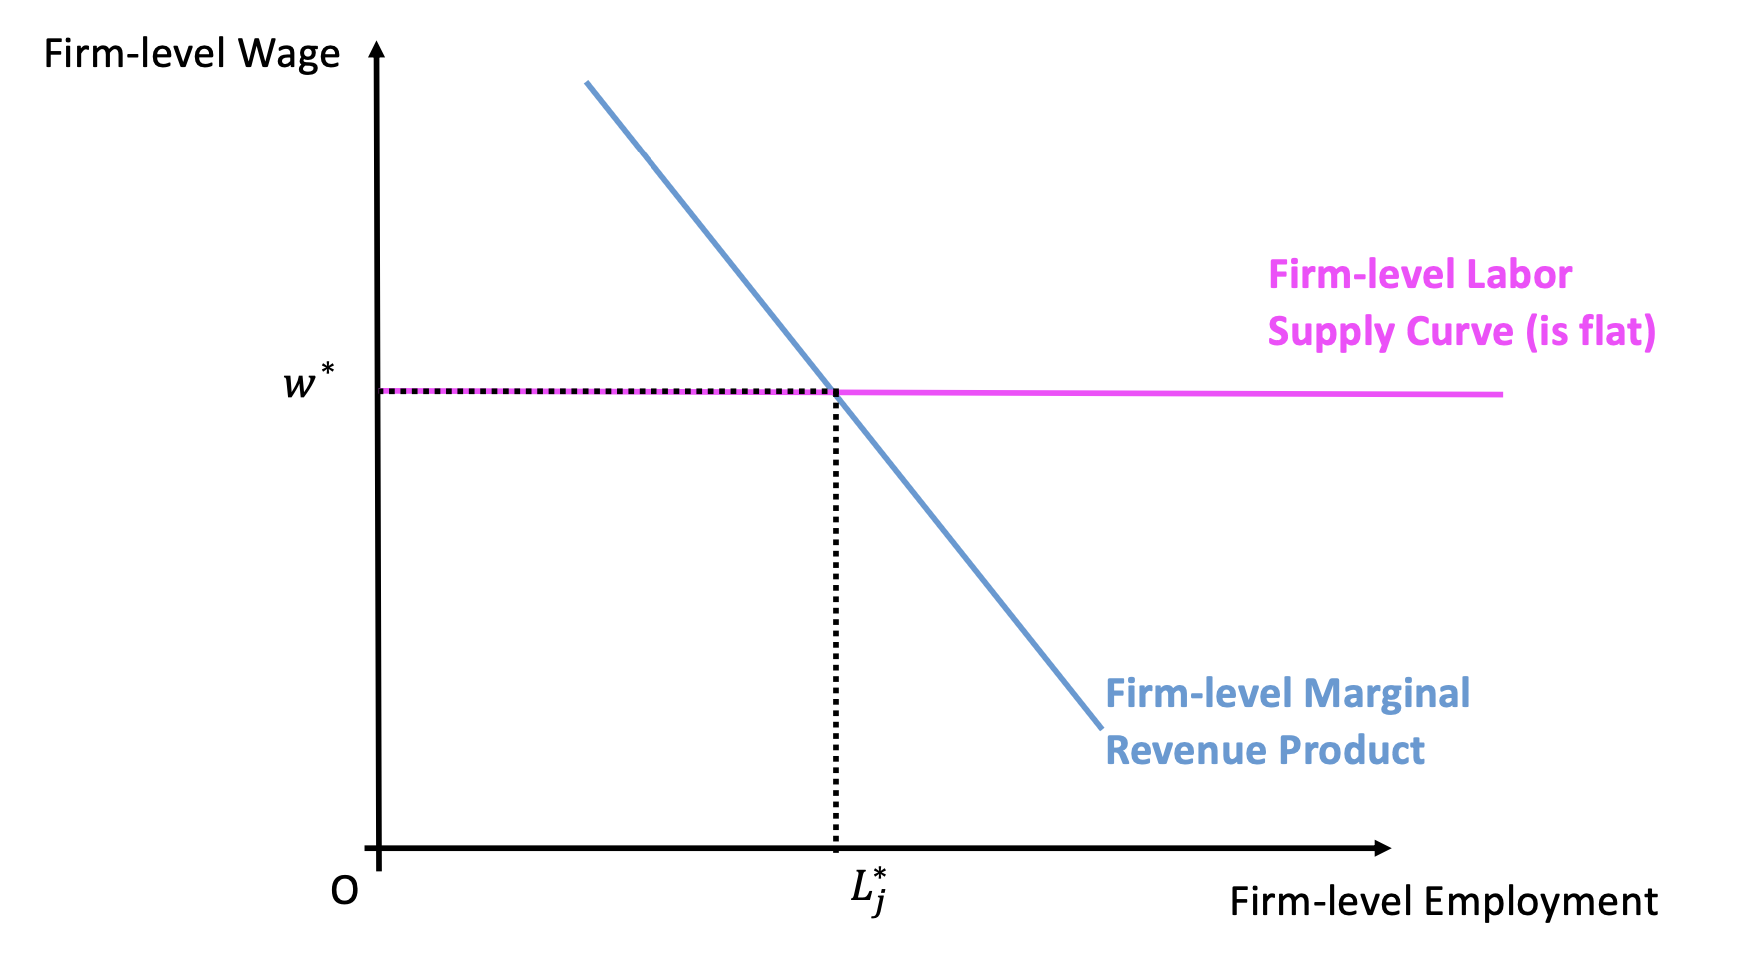
\includegraphics[width=4in]{images/ch2/neoclassical_1.png}
            \caption{Neoclassical Model: Firm's Problem}
        \end{figure}
        \begin{figure}[H]
            \centering
            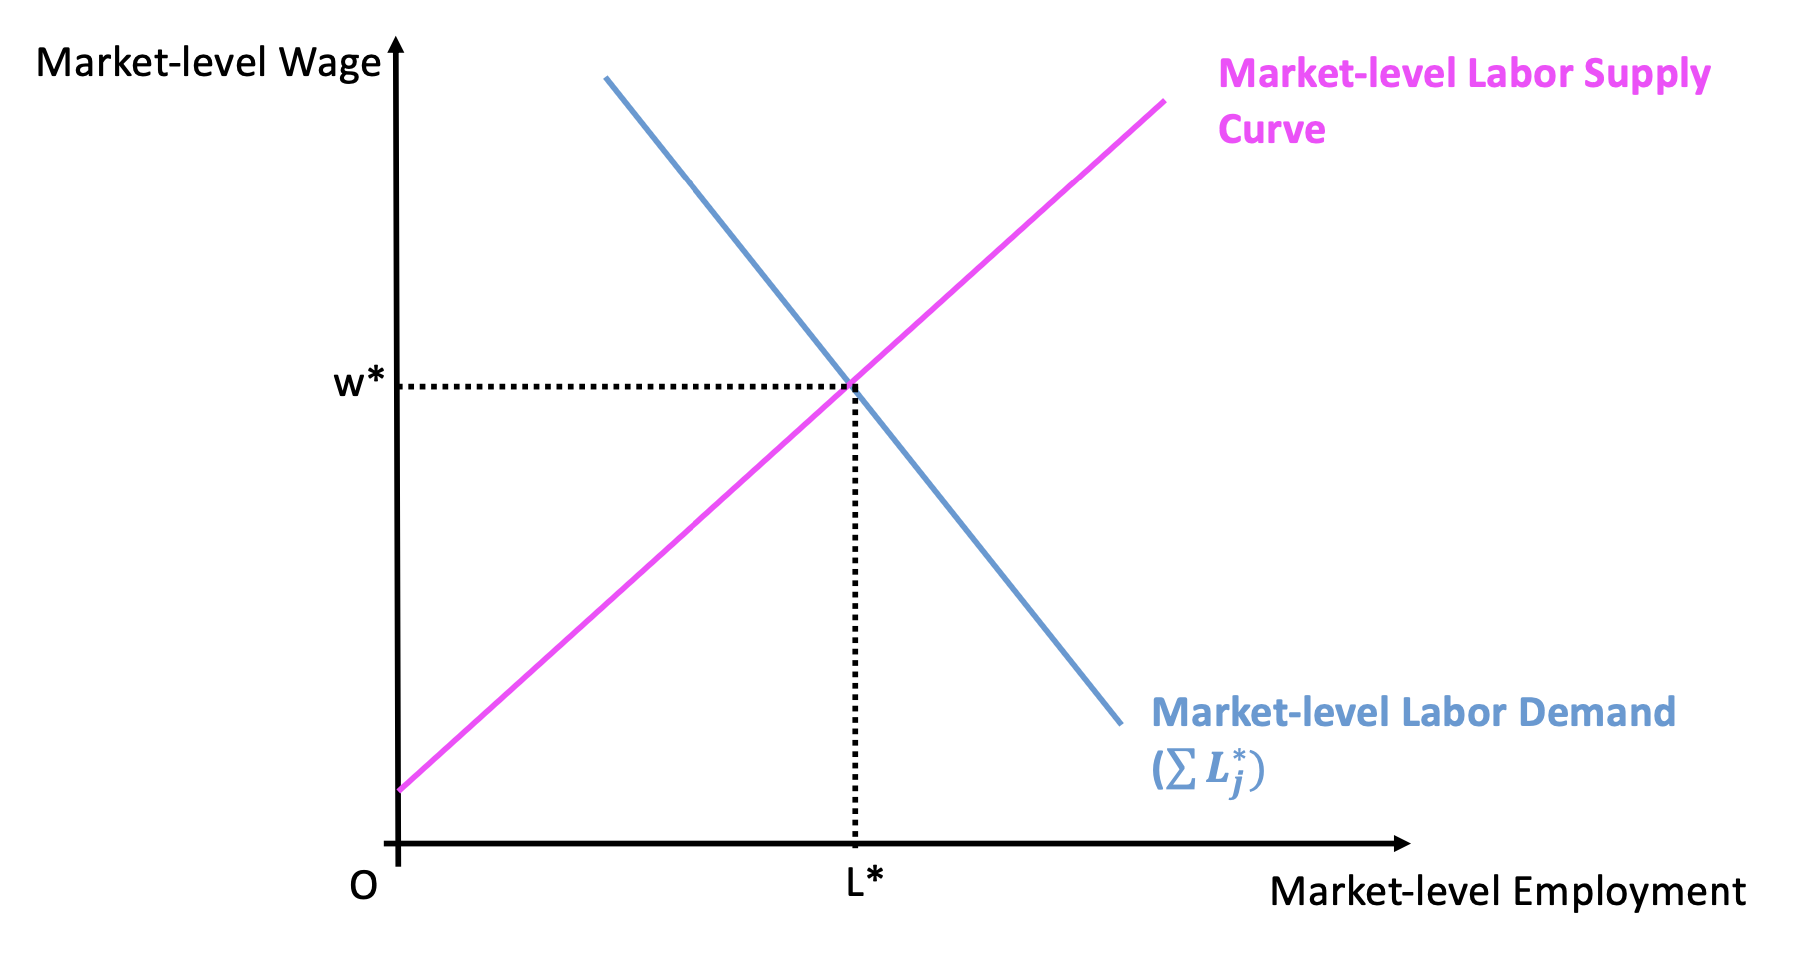
\includegraphics[width=4in]{images/ch2/neoclassical_2.png}
            \caption{Neoclassical Model: Market Equilibrium}
        \end{figure}
        
    \subsection{Effect of Minimal Wage}
        At firm's level, \empha{a minimal wage above equilibrium induces decrease in employment}:
        \begin{figure}[H]
            \centering
            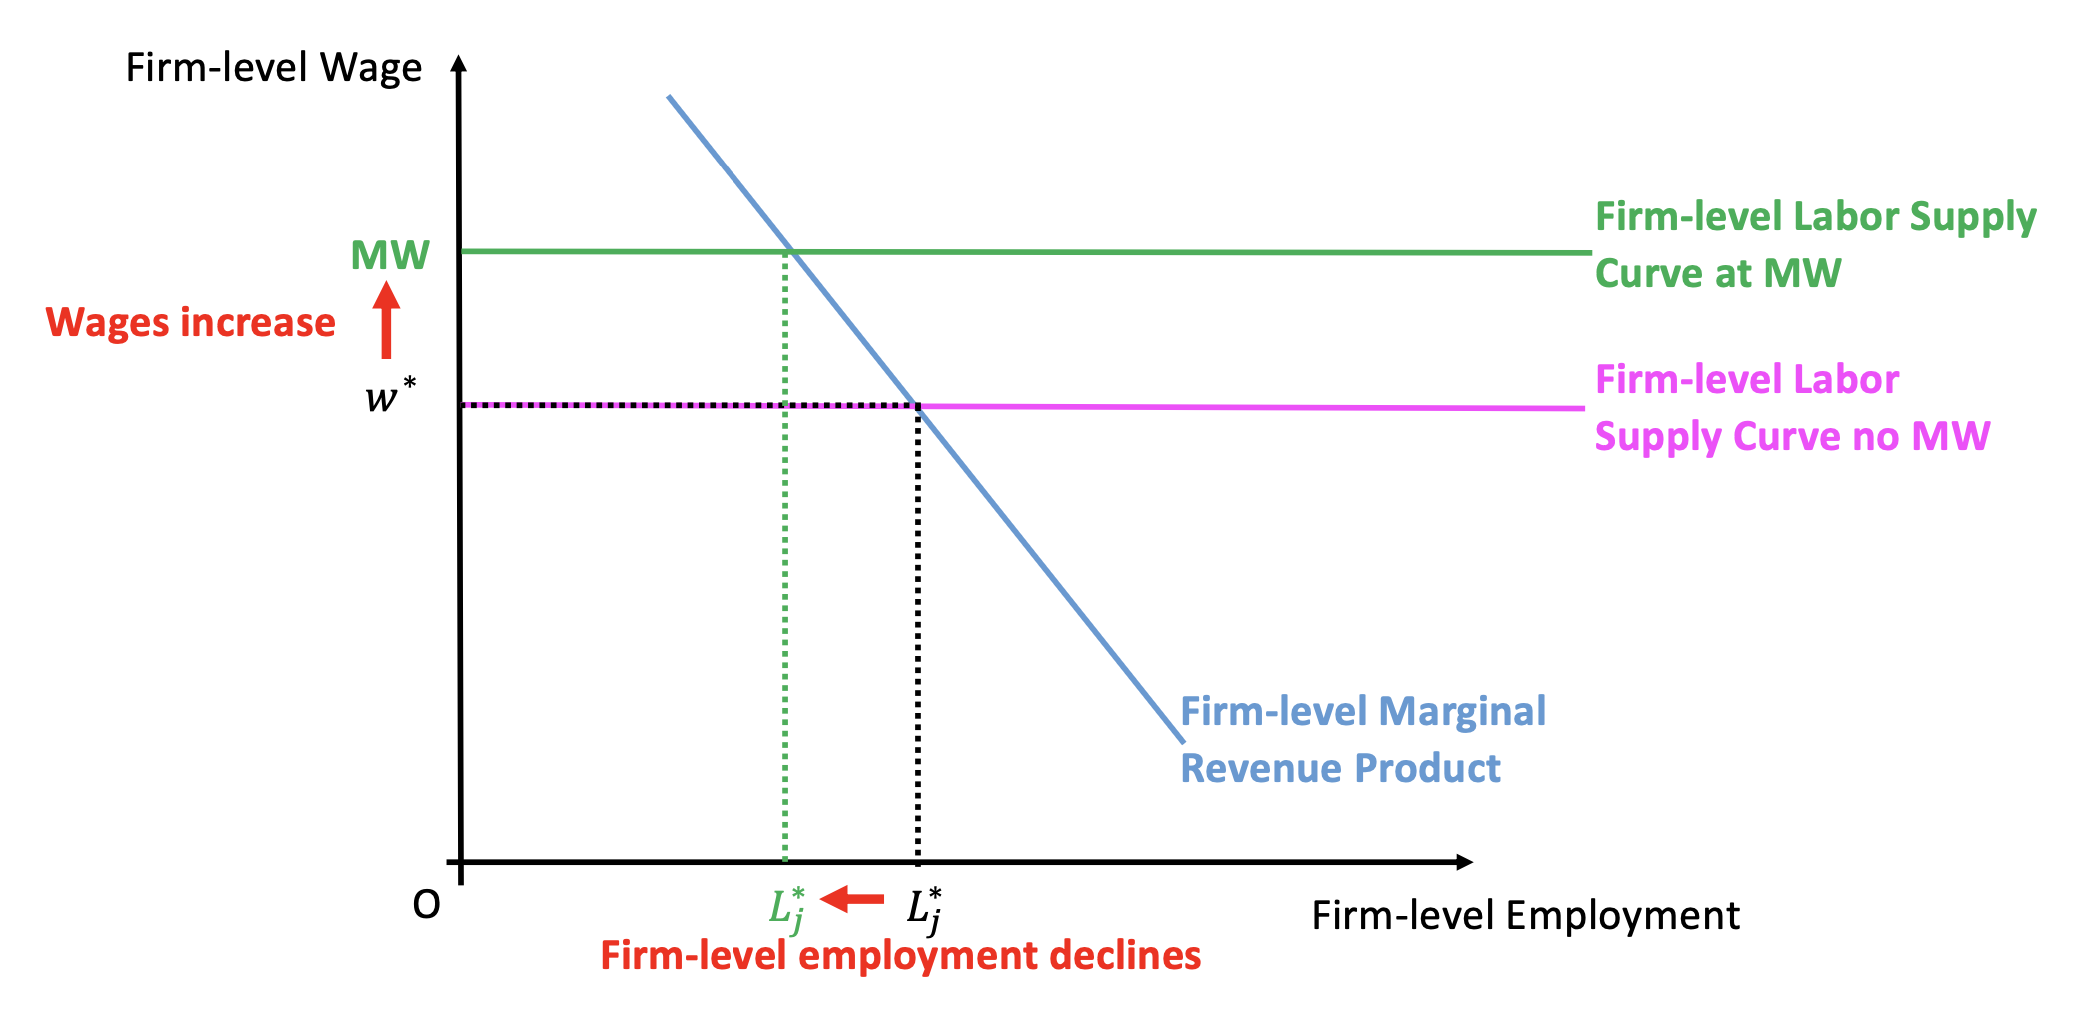
\includegraphics[width=4in]{images/ch2/neoclassical_3.png}
            \caption{Minimal Wage: Firm's Response}
        \end{figure}
        At market level, this causes a welfare loss:
        \begin{figure}[H]
            \centering
            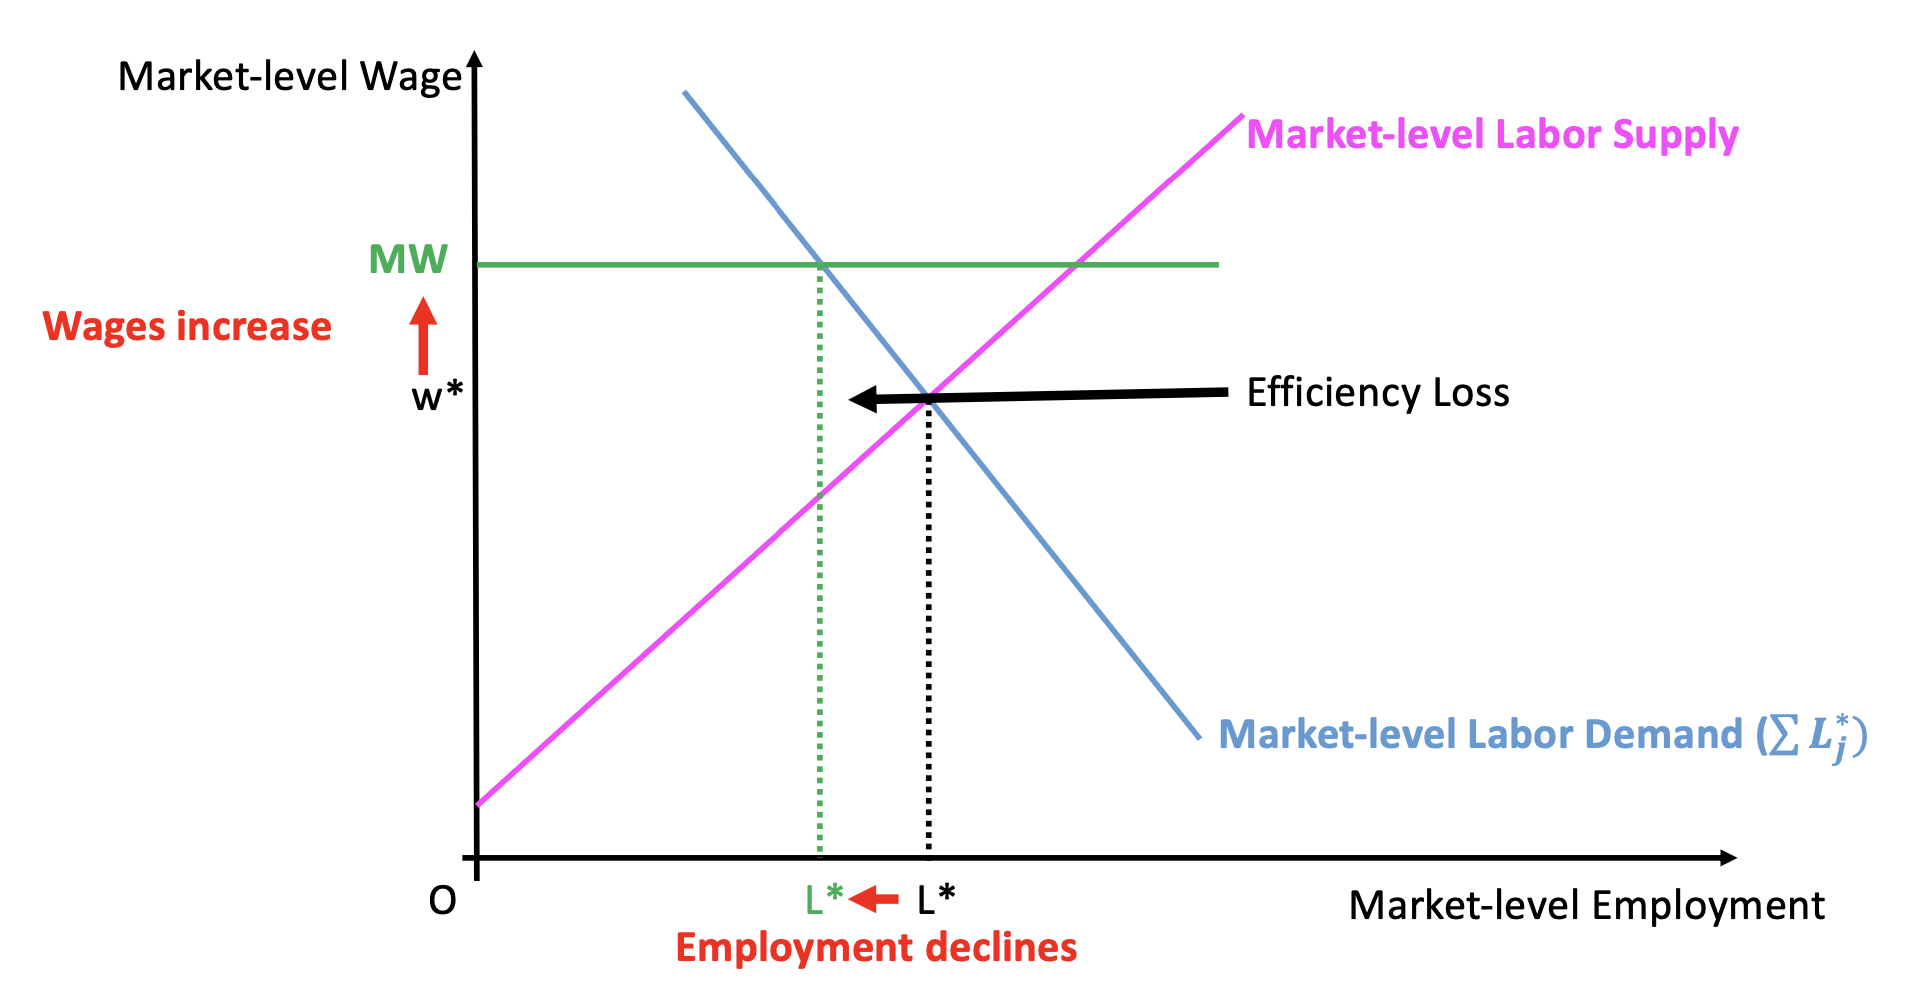
\includegraphics[width=4in]{images/ch2/neoclassical_4.png}
            \caption{Minimal Wage: Market Equilibrium}
        \end{figure}
    
    \subsection{Debate over the Neoclassical Model and the Consensus}
    
        \subsubsection{George Stigler (1946): Price Theory}
            \begin{itemize}
                \item There is no free lunch
                \item Minimum wage decreaes employment and leads to efficiency loss
                \item (This is a testable prediction)
            \end{itemize}
            
        \subsubsection{Richard Lester (1947): Common Sense Approach}
          \begin{itemize}
              \item Abandoned the model and looked at data instead
              \item Ask managers about what determines employment
              \item Most important factor mentioned in responses: demand of output
              \item Less than 20\% reported labour cost as the most important factor
              \item Conclusion: (small) increase in labour cost will have a limited effect on employment
          \end{itemize}
          
        \subsubsection{The Consensus: Milton Friedman (1953): “Essays in Positive Economics”}
            \begin{itemize}
                \item Assumptions can be unrealistic and simplifying
                \item A good model focuses on the most important mechanisms, instead of discussing all irrelevant ingredients
                \item A good model can explain and predict what happens if circumstances change
                \item Evidence produced over the 60-80s supports declining employment
                \item \textbf{Consensus}: Chicago-style approach/price theory captures what happens in response to a minimum wage
            \end{itemize}
    
\section{Consensus Breaks: Modern Empirical Evidences}

    \subsection{Card and Krueger (1994, 1995) and the “Credibility Revolution”}
    
        \subsubsection{Card and Krueger (1994, 1995)}
            Card and Krueger (1994, 1995) studied the impact of an increasing minimum wage in New Jersey with a Difference-in-Difference approach. Their control group is Pennsylvania where there was no minimum wage hike. Their results showed that the increase in minimum wage \empha{increased both wages and employment} in New Jersey. This contradicted the neoclassical model.
            \begin{itemize}
                \item Their DiD design:
                $$\Delta E_i = \alpha + \beta 'X_i + \gamma NJ_i + \epsilon_i$$
                where $X_i$ controls for store characteristics and $NJ_i$ is a dummy takes value 1 for New Jersey.
                \item Their Exposure design:
                $$\Delta E_i = \Tilde{\alpha} +\Tilde{\beta} 'X_i +\Tilde{\gamma} GAP_i + \Tilde{\epsilon}_i$$
                where $GAP_i = NJ_i \times \max \left\{\frac{5.05 - W_{1,i}}{W_{1,i}},0\right\}$ accounts for the wage increase due to the policy.
            \end{itemize}
            Results:
            \begin{figure}[H]
                \centering
                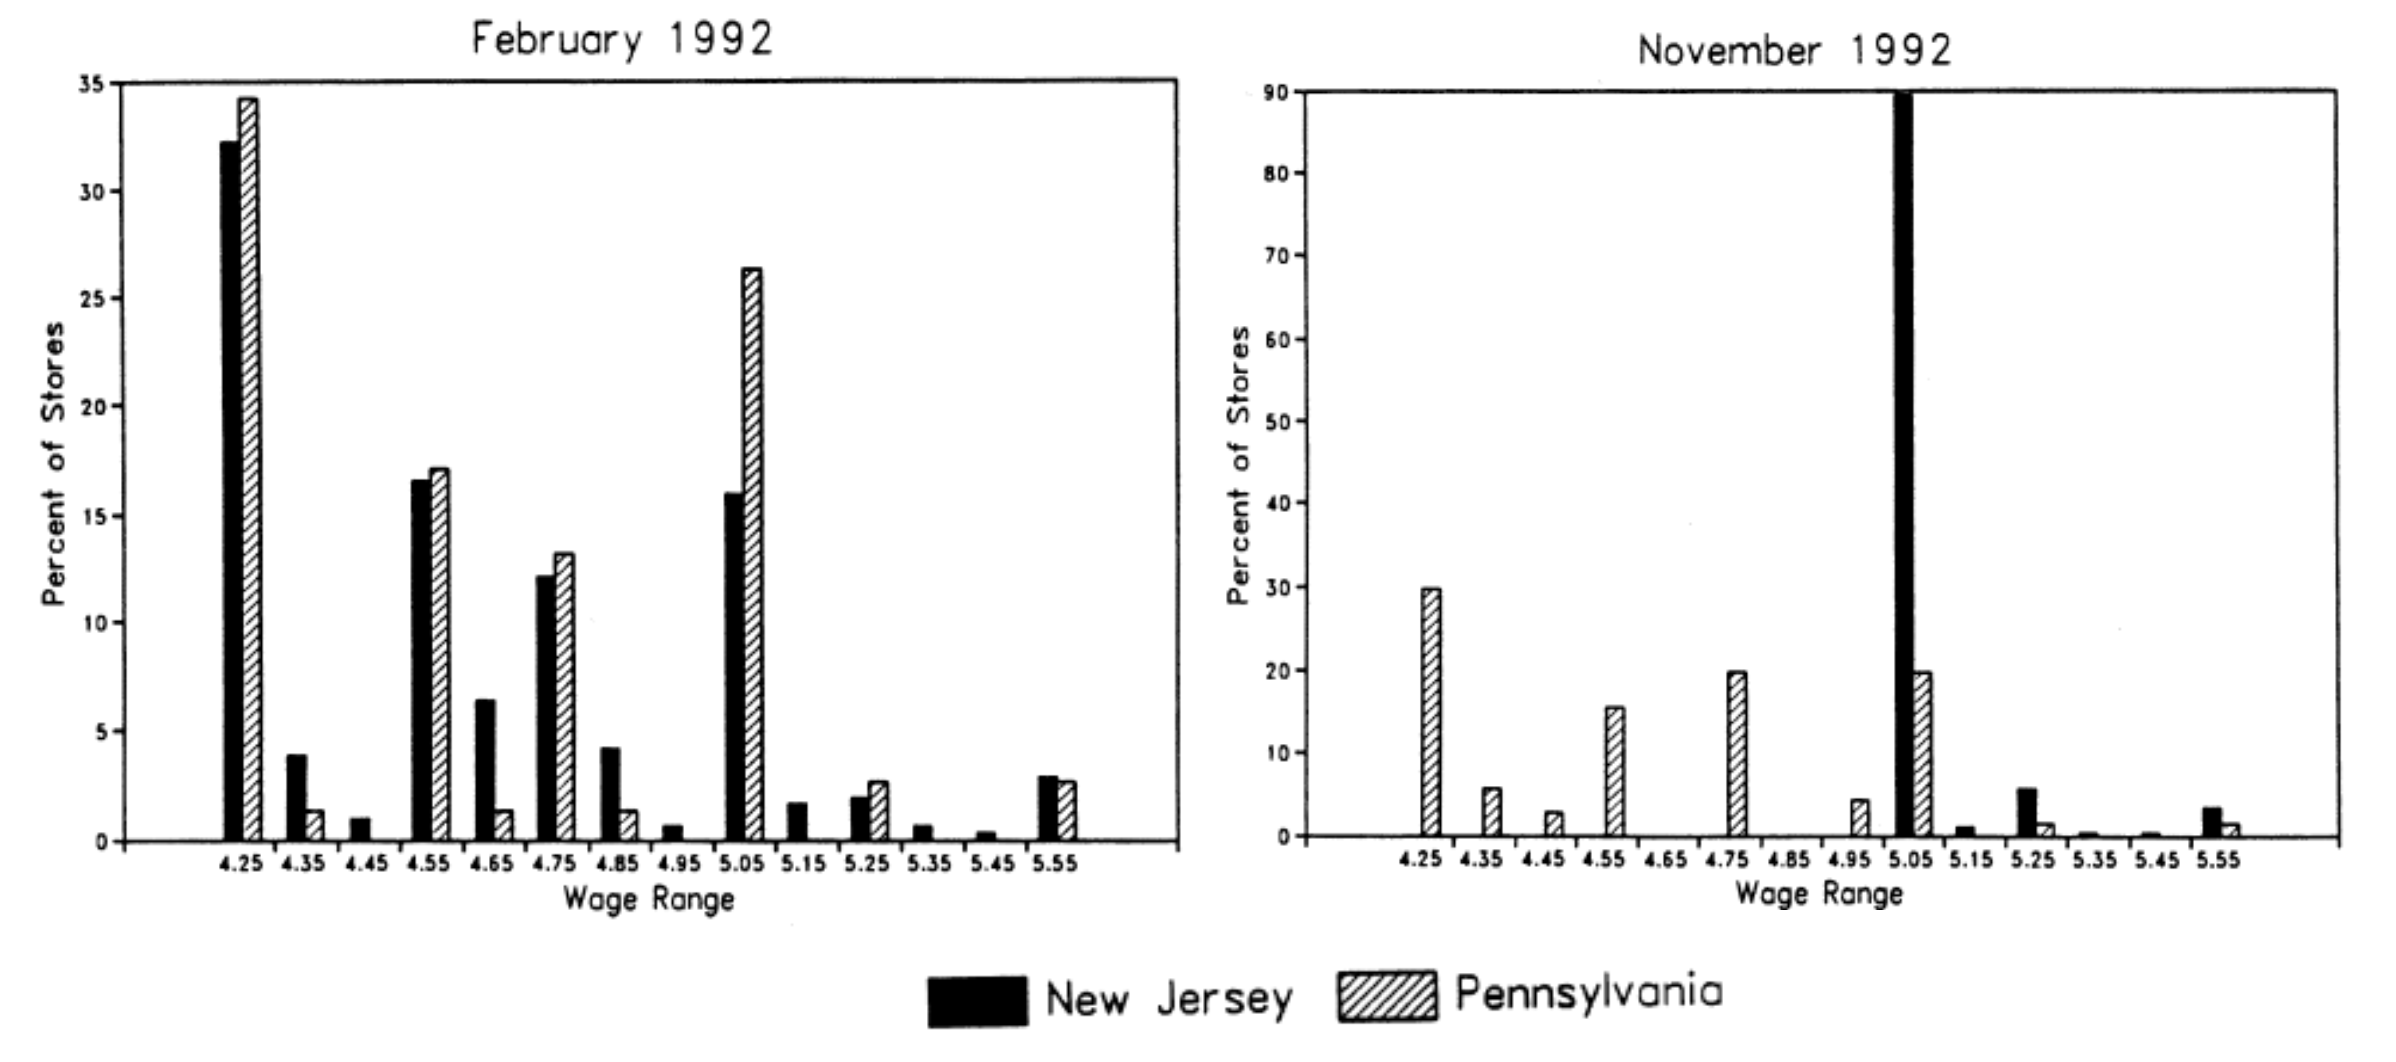
\includegraphics[width=5in]{images/ch2/New Jersey.png}
                \caption{Wage Distributions}
            \end{figure}
            \begin{figure}[H]
                \centering
                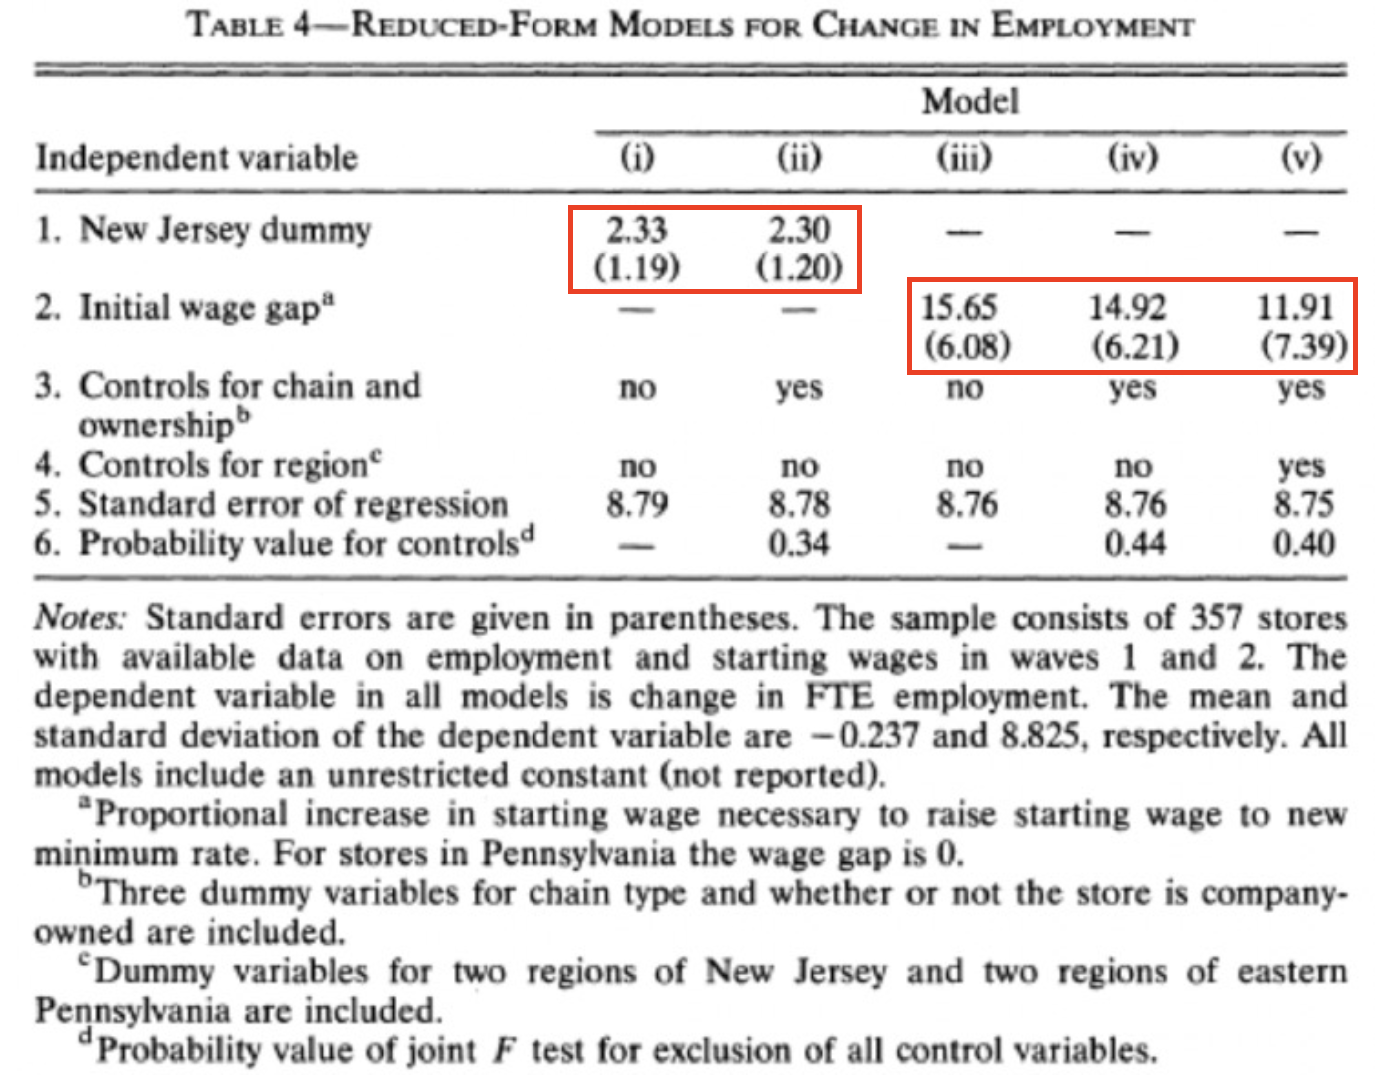
\includegraphics[width=4in]{images/ch2/New_Jersey 2.png}
                \caption{1st Row: DiD; 2nd Row: Exposure Design}
            \end{figure}
            Their results provided clear evidence that the increase in minimum wages in New Jersey caused an increase in both wages and employment.
            
        \subsubsection{A Lesson Learnt for Economists}
            \begin{itemize}
                \item Economic models are important as they can capture the most important mechanisms at play
                \item Simplicity is value, but we should not be dogmatic about our models
                \item We need “credible” research designs, that could be used to reject or accept the key predictions of our models
                \item Alan Krueger (2018): “The idea of turning economics into a true empirical science, where core theoriescan be rejected, is a BIG, revolutionary idea.”
            \end{itemize}
    
    \subsection{New Mimimum Wage Research}
        New minimum wage research shifted the focus from theory to \emphb{"reduced form"} empirical evidence on employment and wages, investigating the impact of minimum wages directly.
        
        The U.S. has been a fertile ground due to state-level variations that can be exploited:
        \begin{itemize}
            \item Two-way Fixed Effects estimation (e.g. Neumark and Wascher, 1993)
            \item Usage of administrative data (e.g. Card and Krueger, 2000)
            \item Border-discontinuity design (e.g. Dube, Lester and Reich, 2010)
        \end{itemize}
        
        On the other hand, most of the evidence focuses on specific demographic groups (e.g. teens) or sectors (e.g. restaurants). It could be possible that minimum wages increase employment in some sectors but decrease it in others.
        
    \subsection{Frequency Distribution Based Approach}
        \subsubsection{Idea}
        Cengiz et al. (2019) develop a novel method to assess the overall employment change using changes in distribution:
        \begin{figure}[H]
            \centering
            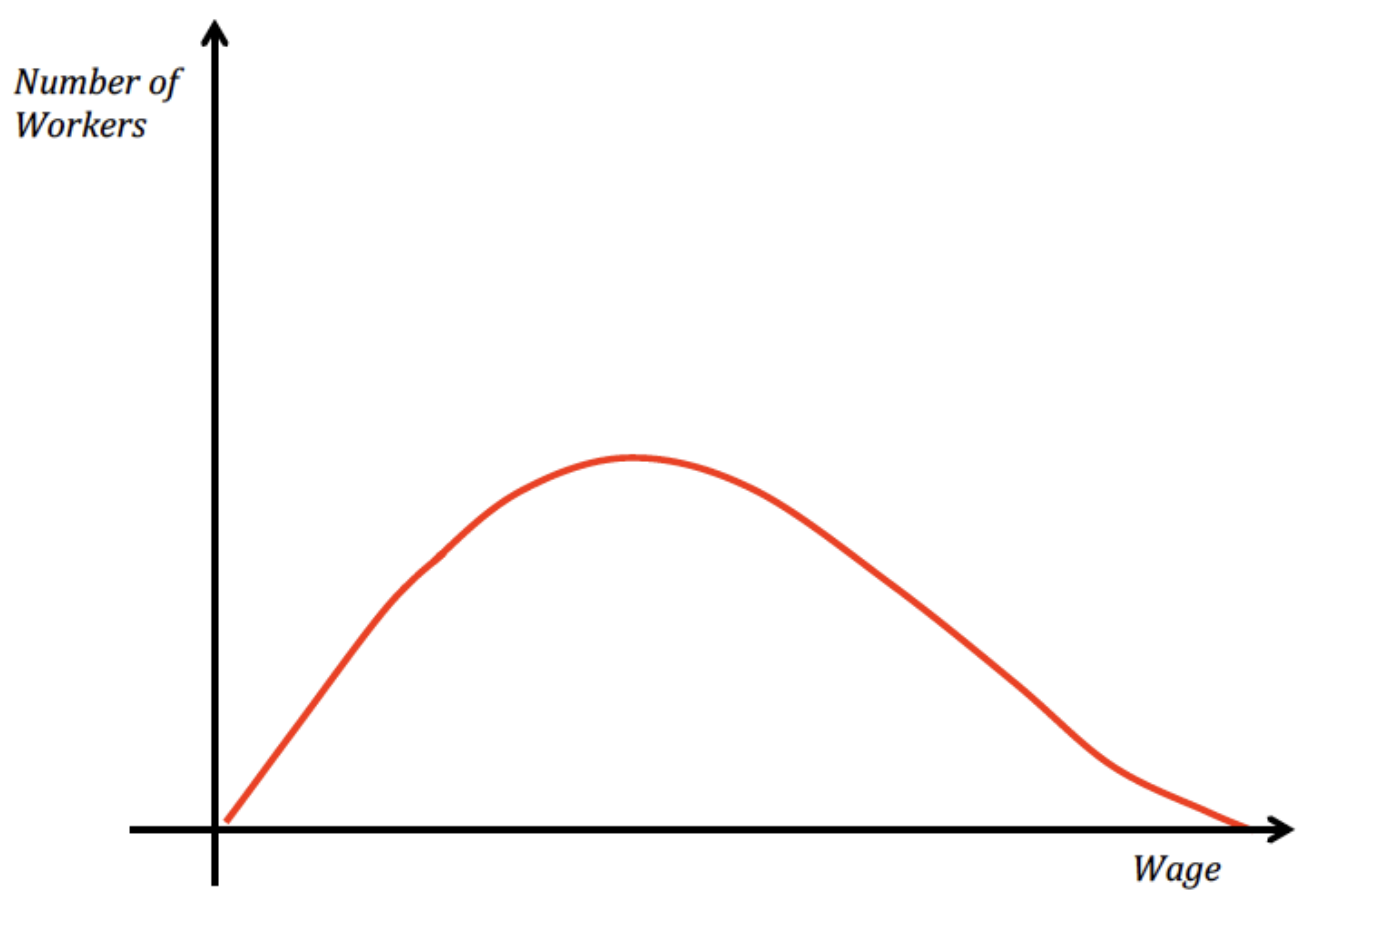
\includegraphics[width=4in]{images/ch2/Freq_approach_1.png}
            \caption{Distribution of Employment before Policy Change}
        \end{figure}
        After an increase in the minimum wage, jobs with wages below the threshold will disappear and new jobs with wages higher than the threshold will be generated. The net effect on employment is illustrated below:
        \begin{figure}[H]
            \centering
            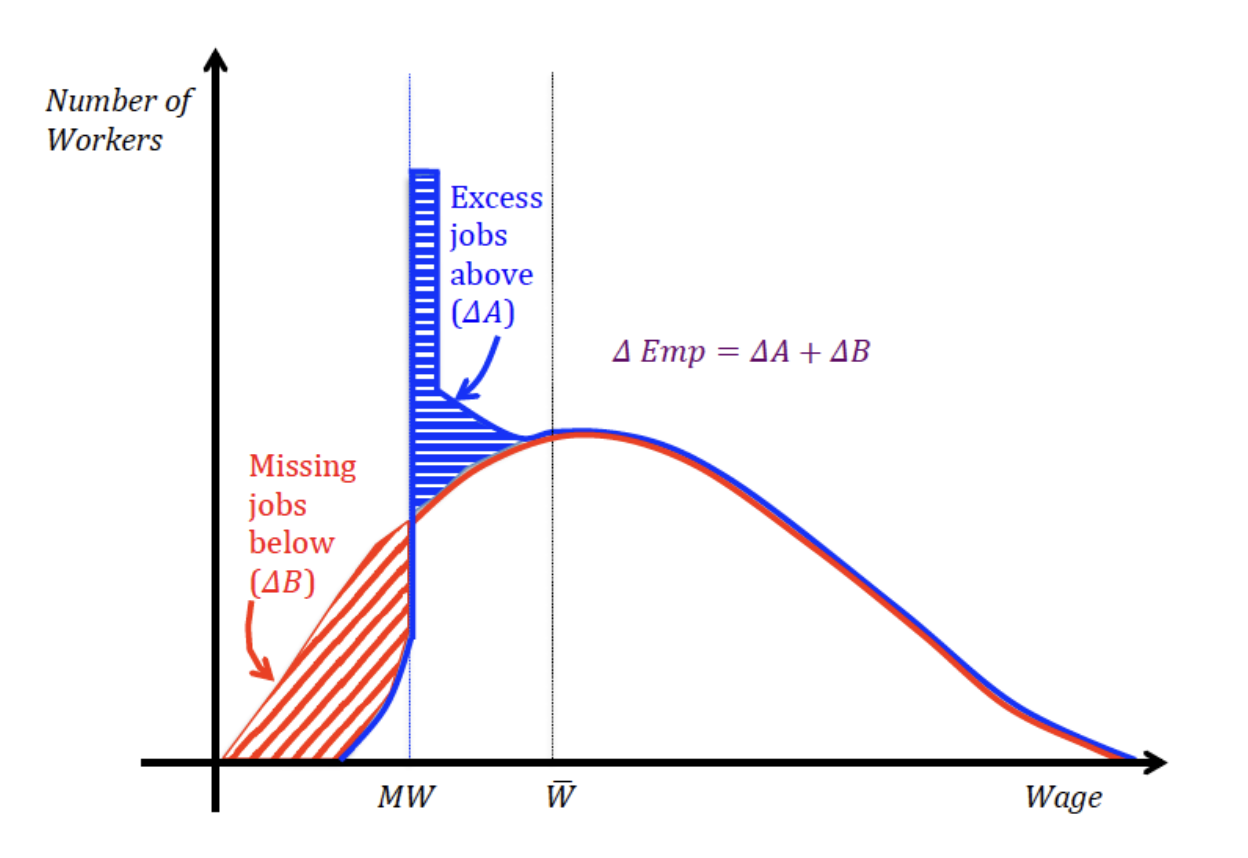
\includegraphics[width=4in]{images/ch2/Freq_approach_2.png}
            \caption{Distribution of Employment after Policy Change}
            \label{fig:freq_approach}
        \end{figure}
        The key empirical challenge of this method is to get counterfactual wage distribution. The solution is to use a DiD idea.
        
        During 1999-2000, Washington State raised its minimum wage from \$7.51 to \$9.18, and WA has administrative data on hourly wages. We divide the distribution by wage bins, and calculate the counterfactual by creating a synthetic control group from a number of states.

        With this method, Cengiz et al. obtained both actual and counterfactual employment distributions:
        \begin{figure}[H]
            \centering
            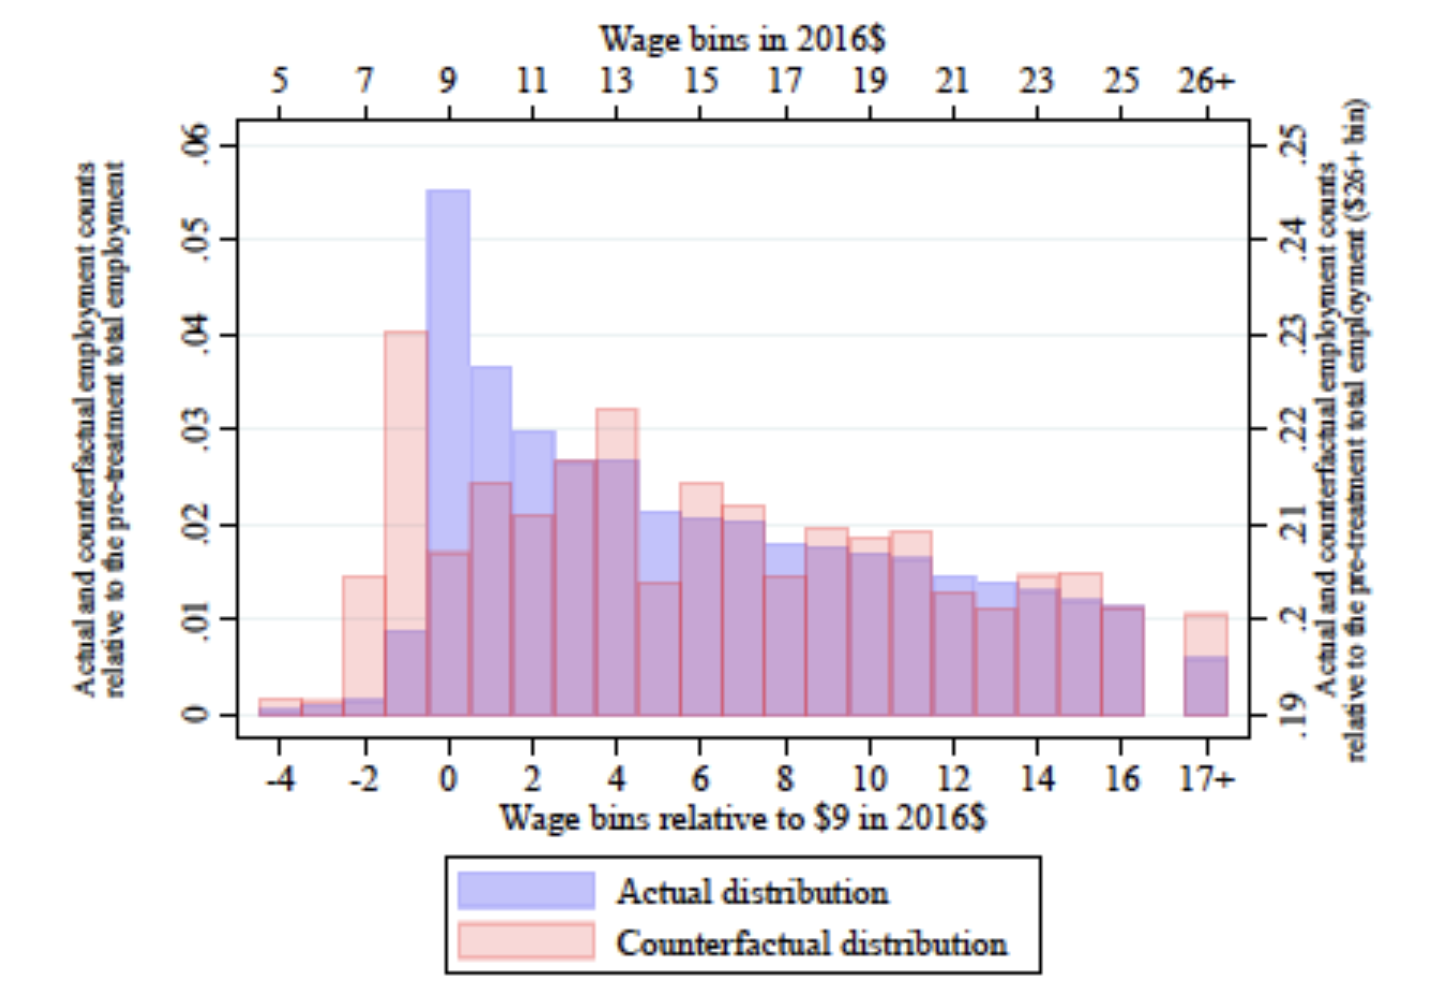
\includegraphics[width=3.5in]{images/ch2/Freq_approach_3.png}
            \caption{Actual and Counterfactual Distributions}
        \end{figure}
        Comparing the two distributions, the effect of an increase in minimum wage is retrieved. The patter of change matches Figure \ref{fig:freq_approach}, and, as shown by the red line, there is a redistribution of employment from jobs with wages below the threshold to jobs with wages above the threshold. No reduction in overall employment is observed:
        \begin{figure}[H]
            \centering
            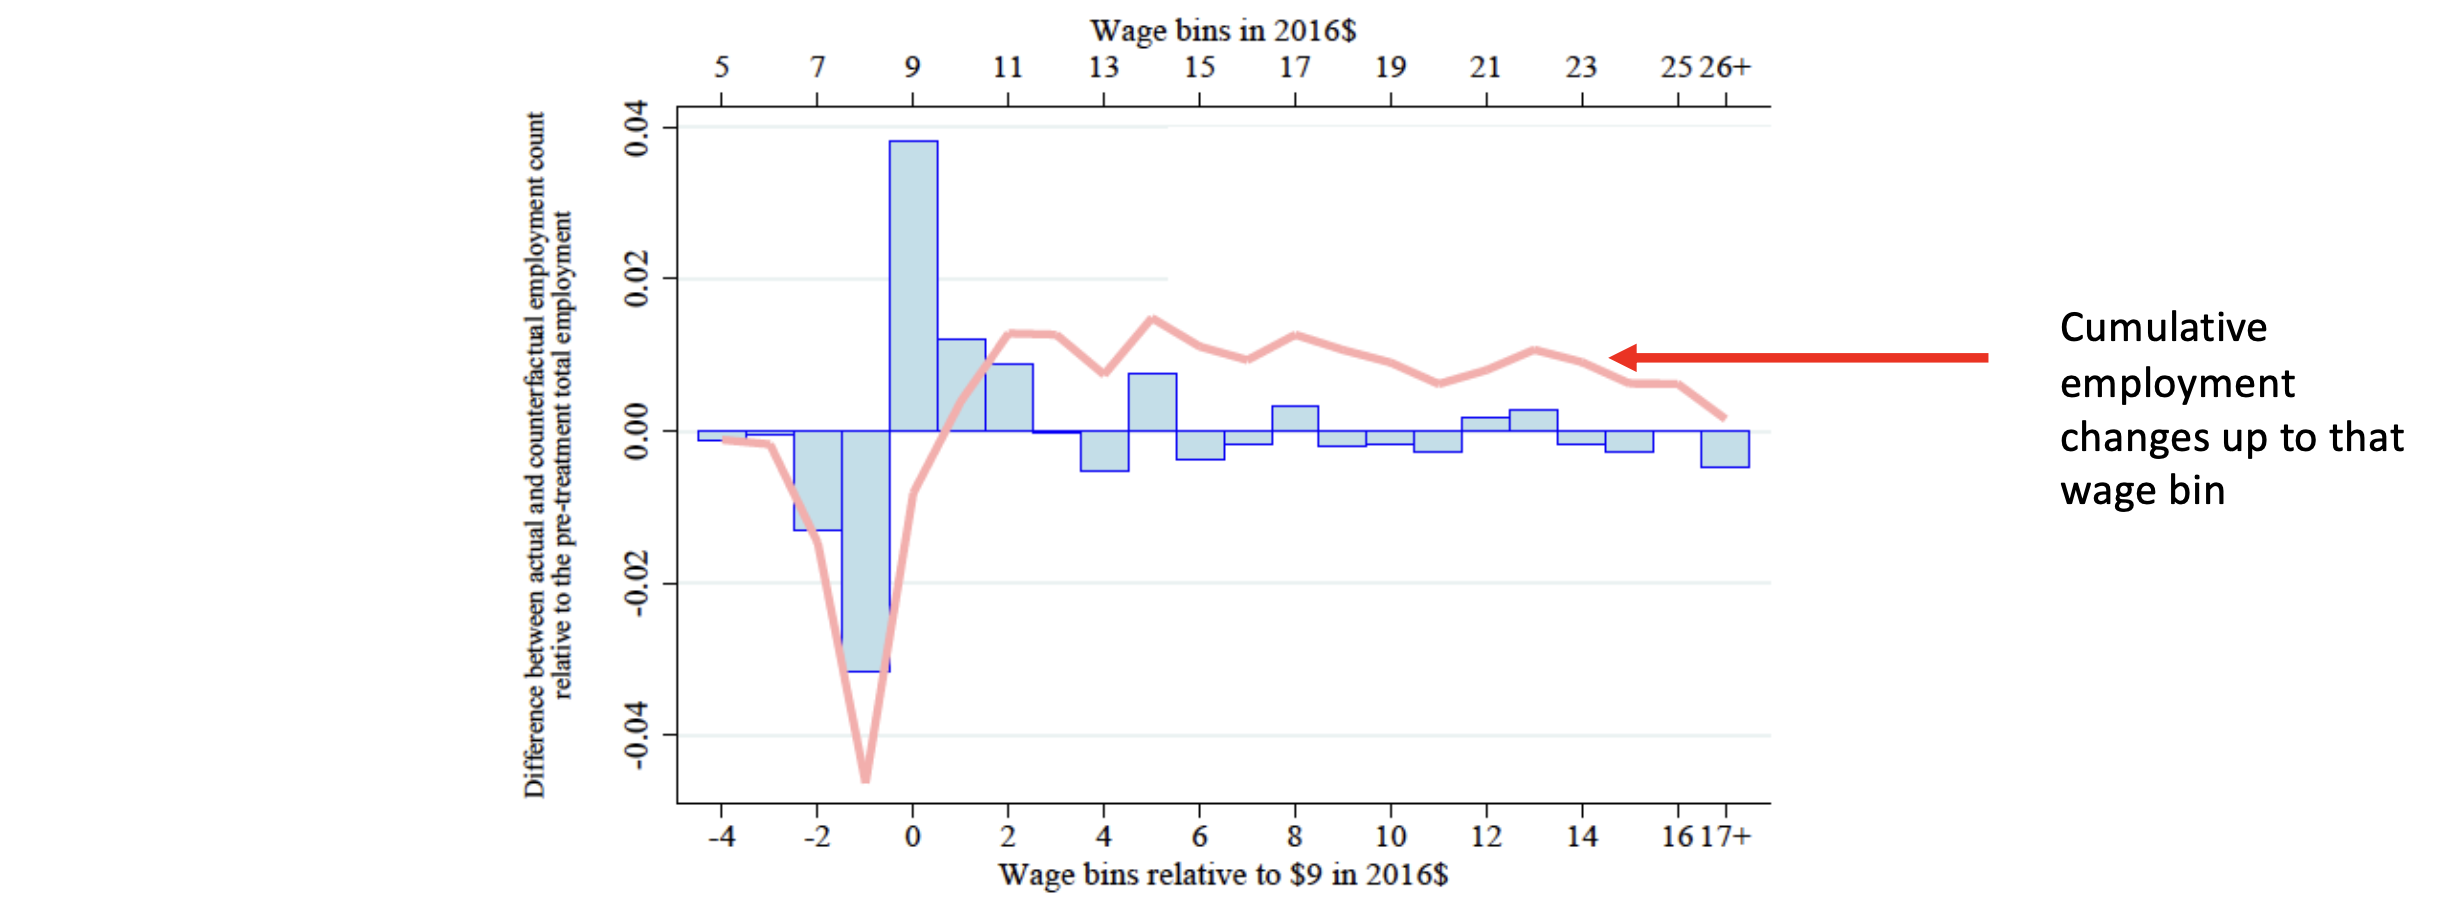
\includegraphics[width=6.5in]{images/ch2/Freq_approach_4.png}
            \caption{Treatment Effect}
        \end{figure}
        Taking heterogeneity into account, we cannot find any overall dis-employment either:
        \begin{itemize}
            \item No evidence that dis-employment effects are more prominent for larger changes
            \begin{figure}[H]
                \centering
                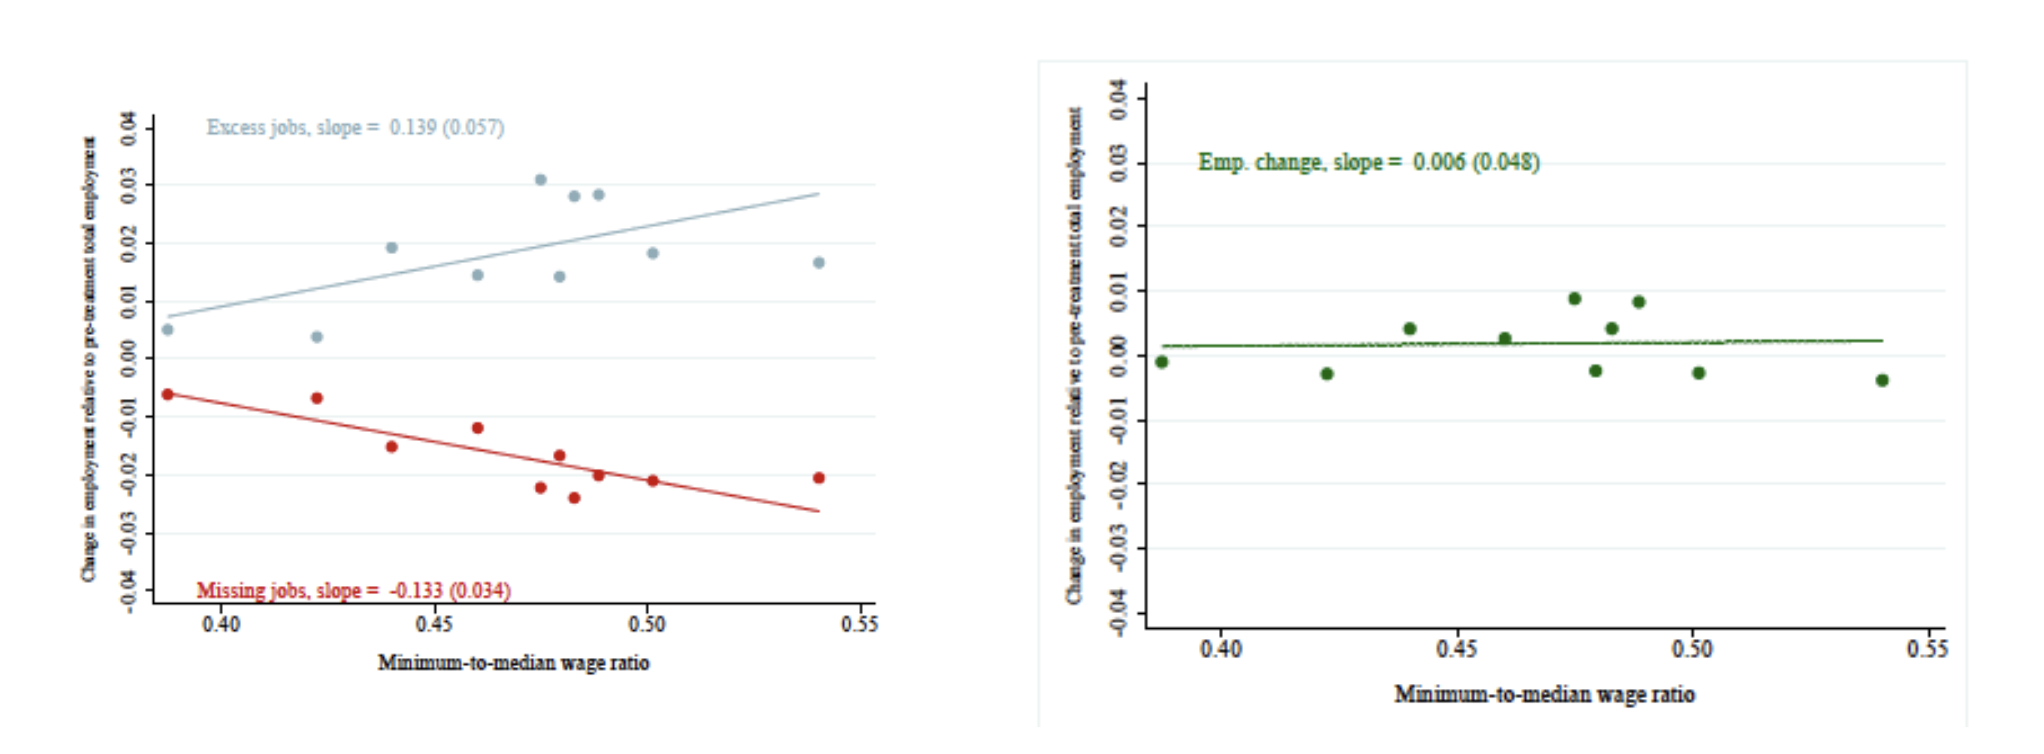
\includegraphics[width=5.5in]{images/ch2/Freq_approach_5.png}
                \caption{Heterogeneity by Magnitude of Increase}
            \end{figure}
            \item No evidence that dis-employment effects are more prominent when unemployment rate is high
            \begin{figure}[H]
                \centering
                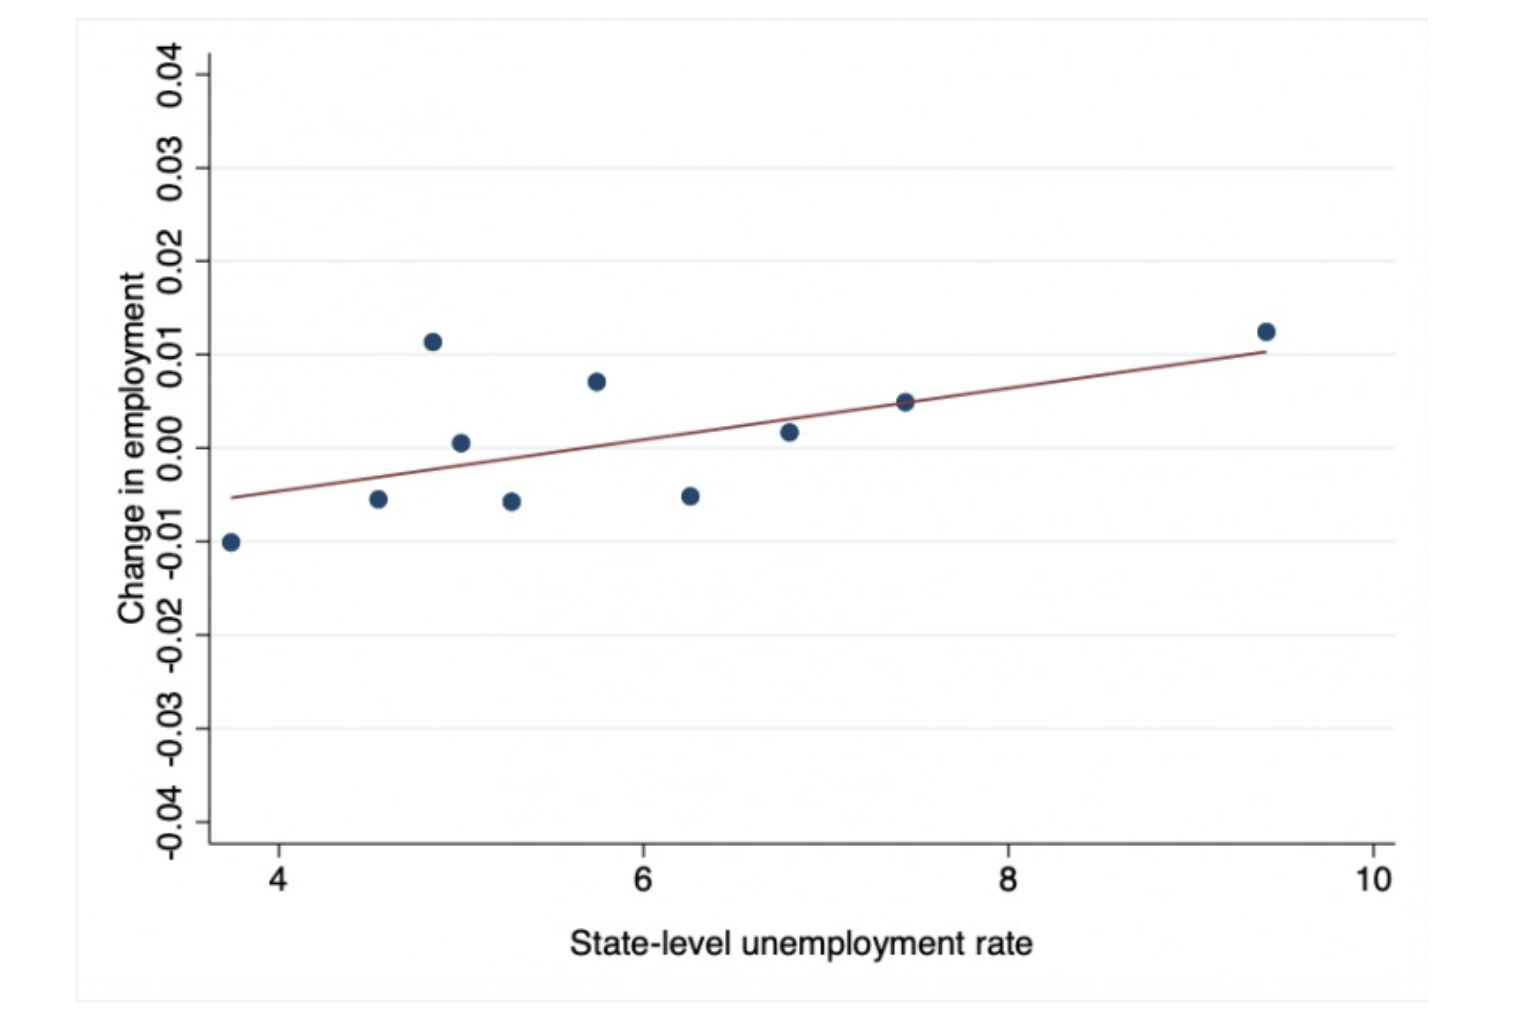
\includegraphics[width=4in]{images/ch2/Freq_approach_6.png}
                \caption{Heterogeneity by State Unemployment Level}
            \end{figure}
        \end{itemize}
        
        
\section{$\star$ Monopsonistic Model}

    \subsection{Firm's Problem and Equilibrium}
    
        \subsubsection{Assumptions}
            Empirical research presented in the previous section show no evidence that an increase in minimum wage will cause dis-employment. This indicates that assumptions we made for the standard neoclassical ``price theory'' model do not hold. In reality:
            \begin{itemize}
                \item Workspaces are differentiated (not homogeneous)
                \item Such differentiation provides each employer with some market power
                \item The labour market is a \emphb{monopsonistic market}
            \end{itemize}
            The intuition is that, because some workers want to work at a certain firm, the employer can hire them with lower wages. This creates a wedge between productivity and wages. In equilibrium, fewer workers are hired and wages are lower.
            
        \subsubsection{Firm's Optimisation Problem}
            Firms maximise their profits:
            $$\max_{L_j} pf(L_j) - w(L_j)L_j$$
            The FOC implies that:
            $$\color{red} \underbrace{pf'(L_j)}_{\text{Marginal\ Revenue\ Product}} = \underbrace{w(L_j)\left(1+\frac{1}{\eta}\right)}_{\text{Marginal\ Cost}}$$
            where $\eta$ is the \emphb{elasticity of firm-level labour supply} defined as $\eta = \frac{\partial L_j}{\partial w}\frac{w}{L_j} > 0$.
            The \emphb{equilibrium wage} in monopsonistic model is:
            $$\color{red} w^*(L_j)= \underbrace{pf'(L_j)}_{\text{Marginal\ Revenue\ Product}} \times \underbrace{\frac{1}{1+\frac{1}{\eta}}}_{\text{Mark-down}(<1)} < w^*_{Neoclassical}$$
            The equilibrium wage here is different from the marginal revenue product: firms enjoy a "\emphb{markdown}." The magnitude of such difference depends on firm-level elasticity of labour supply: if $\eta \rightarrow \infty$, we get back to the neoclassical framework.
            \begin{figure}[H]
                \centering
                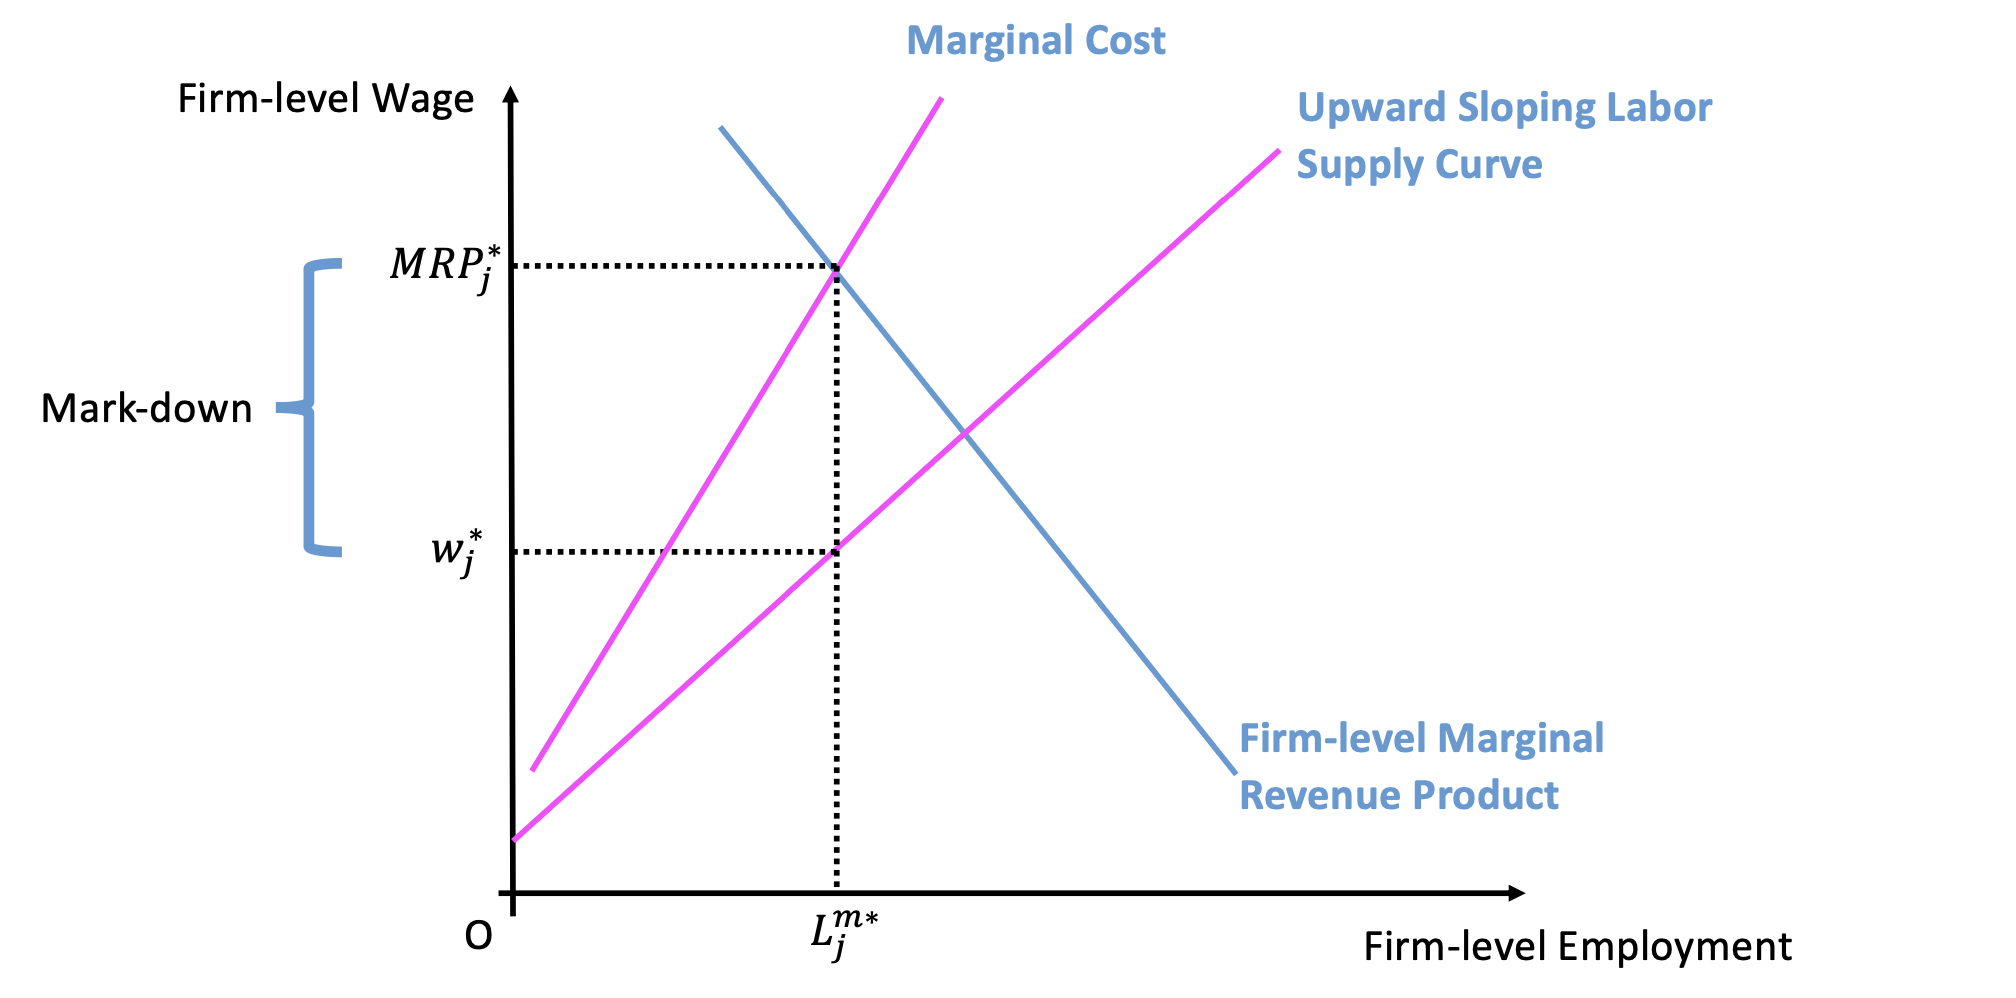
\includegraphics[width=5in]{images/ch2/Monop_LM_1.png}
                \caption{Equilibrium in a Monopsonistic Labour Market}
            \end{figure}
            
        \subsubsection{Predictions}
            Several main predictions of this monopsonistic model:
            \begin{itemize}
                \item People feel they are underpaid at their workplace relative to their true productivity – wages are “marked-down”
                \item People feel they could find a better paying workplace, but those are not ideal (they are too far from home, not nice co-workers)
                \item Workers with similar skills and ability are paid differently at different firms (there is a firm-level skill premium)
                \item Efficient firms are larger and pay more to workers with similar skills
            \end{itemize}
    
    \subsection{Effect of Minimal Wage: Reallocation}
        In this framework, a minimum wage scheme will cause:
        \begin{itemize}
            \item The least efficient firms will close
            \item The most efficient firms increase wages, the mark-down (or profit per worker) falls
            \item Though the wedge between productivity and wage falls, it is still profitable to employ workers
            \item Firms will hire more with lower mark-down
        \end{itemize}
        \begin{figure}[H]
            \centering
            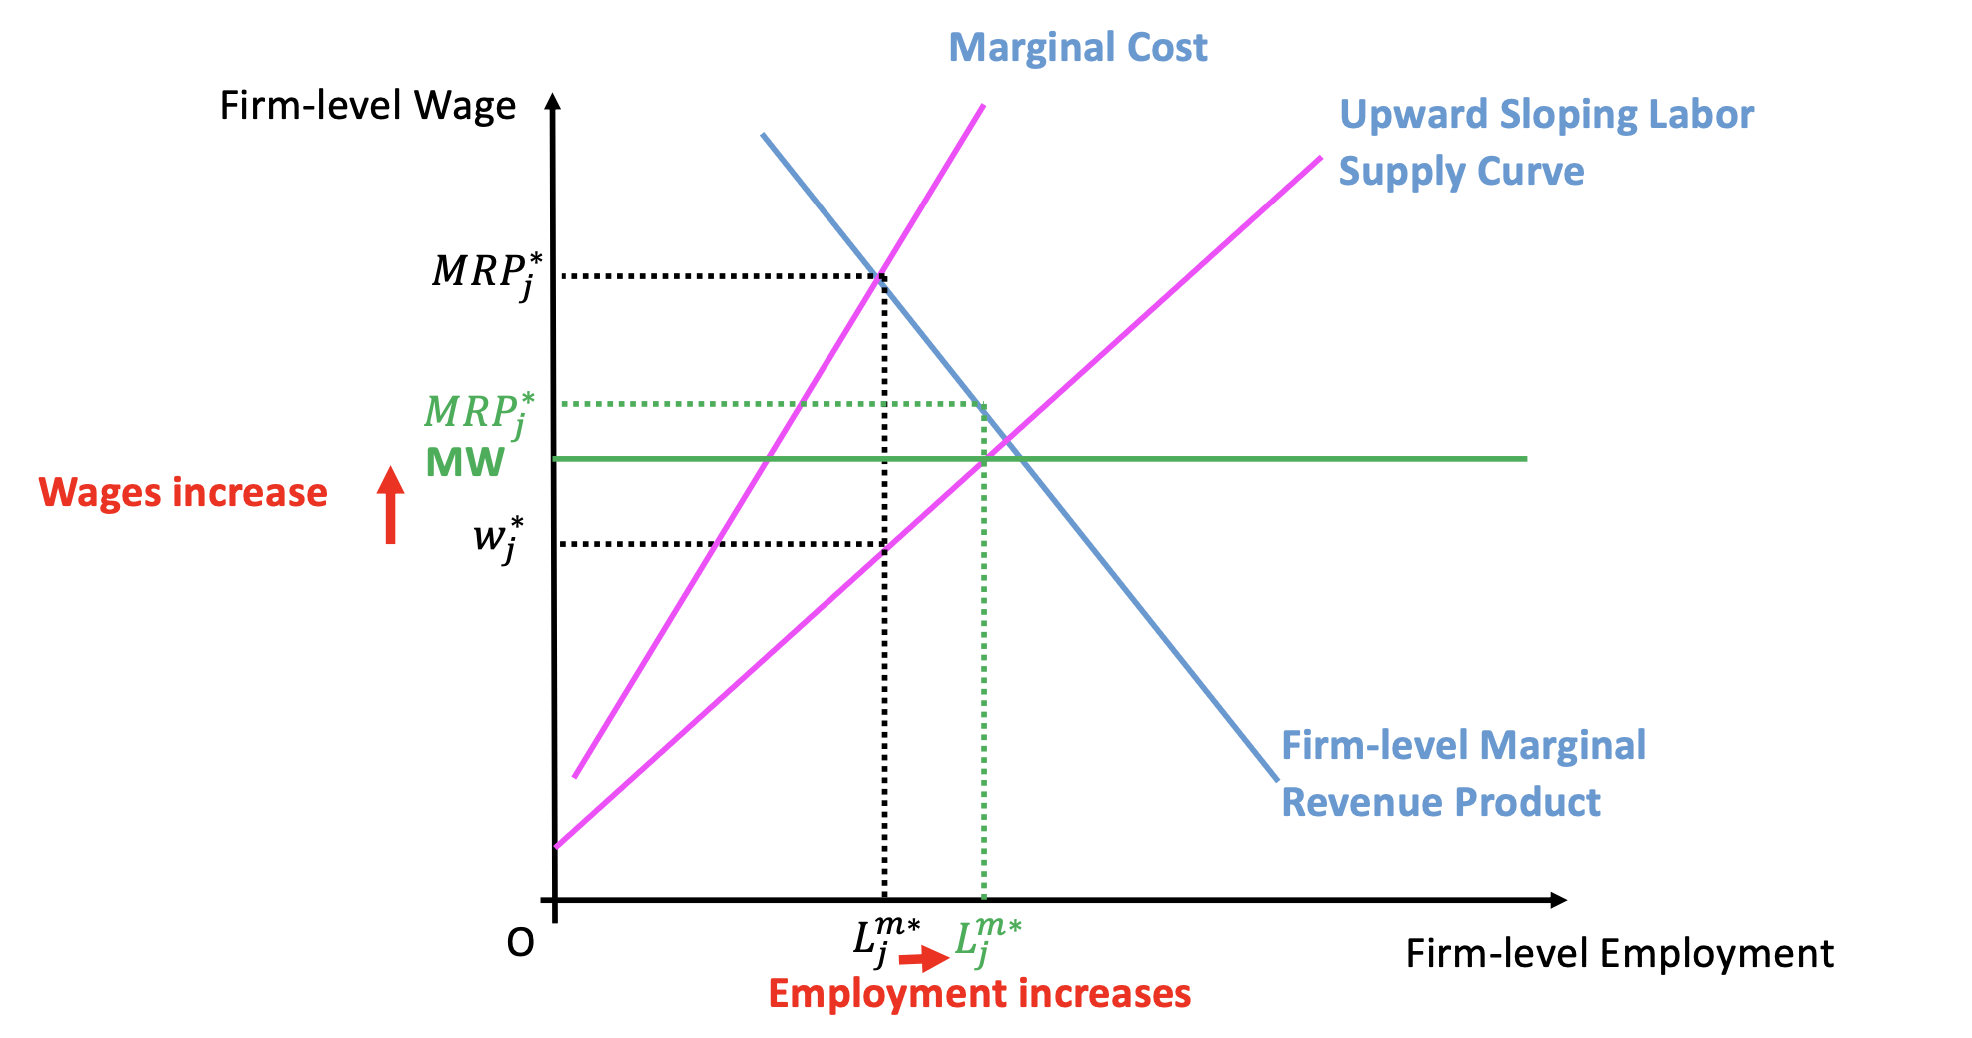
\includegraphics[width=5in]{images/ch2/Monop_LM_2.png}
            \caption{Minimum Wages in Monopsonistic Model}
        \end{figure}
        The overall effect is featured as a process called \emphb{reallocation}: \empha{employees of the least efficient firms are transferred to the more efficient one}. This improves efficiency. Meanwhile, though new firms pay more, workers might be worse off in other aspects, so the overall effect on welfare is still ambiguous.
        
    \subsection{Empirical Research on Reallocation}
        Historically, the role of reallocation has been featured prominently in the minimum wage debate since the later 19th century. (e.g. advocates to use minimum wage to stop the proliferation of "sweatshops" in the 1890s; Winston Churchill's argument for the Trade Boards Act 1909)
        
        \subsubsection{Dustmann, Lindner, Schönberg, Umkehrer, and vom Berge (2022)}
            Dustmann, Lindner, Schönberg, Umkehrer, and vom Berge (2022) provide direct evidence on the impact of the minimum wage on reallocation:
            \begin{itemize}
                \item Reform studied: Introduction of the minimum wage in Germany in 2015
                \item Data: Administrative employer-employee database covering the life history of all German private sector workers
                \item Empirical analysis: How wages, employment, and quality of the firm evolved following minimum wage hikes?
                \item Control groups:
                    \begin{itemize}
                        \item Projection based on the observed trend before the introduction of the minimum wage
                        \item Wage evolution at the higher end of the wage distribution
                    \end{itemize}
            \end{itemize}
            
        \subsubsection{Results}
            Positive wage increases for employees around the minimum wage:
            \begin{figure}[H]
                \centering
                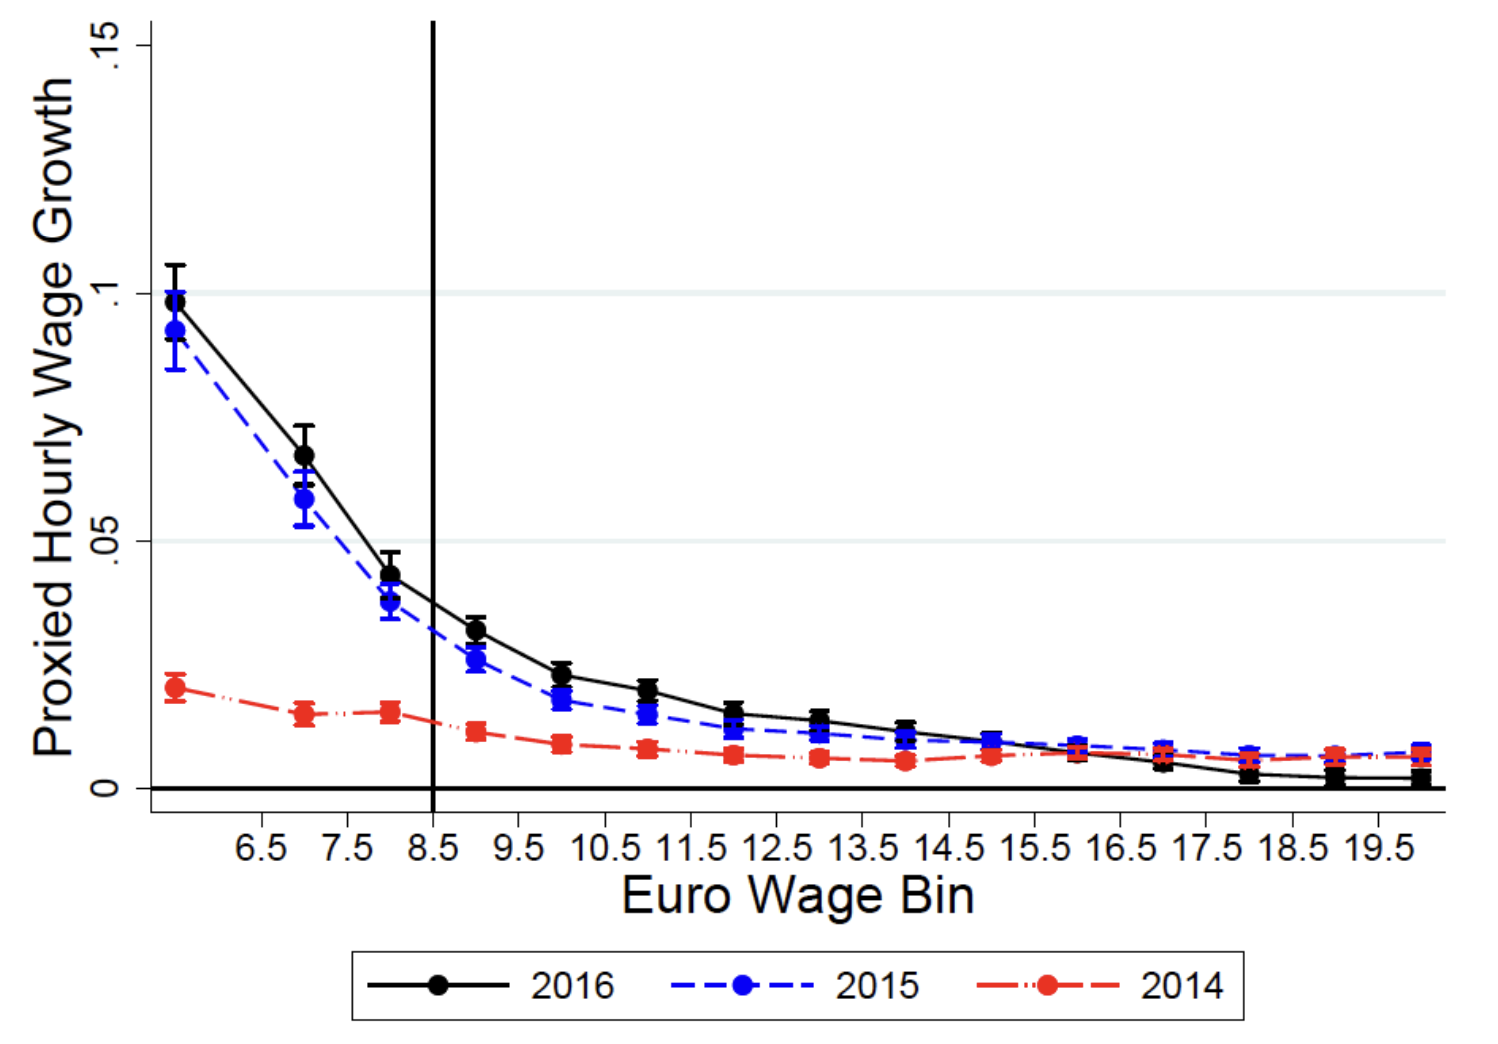
\includegraphics[width=4in]{images/ch2/reallocation_1.png}
                \caption{Wage Growth as a Function of Wages 2 Years Before}
            \end{figure}
            Increase in employment:
            \begin{figure}[H]
                \centering
                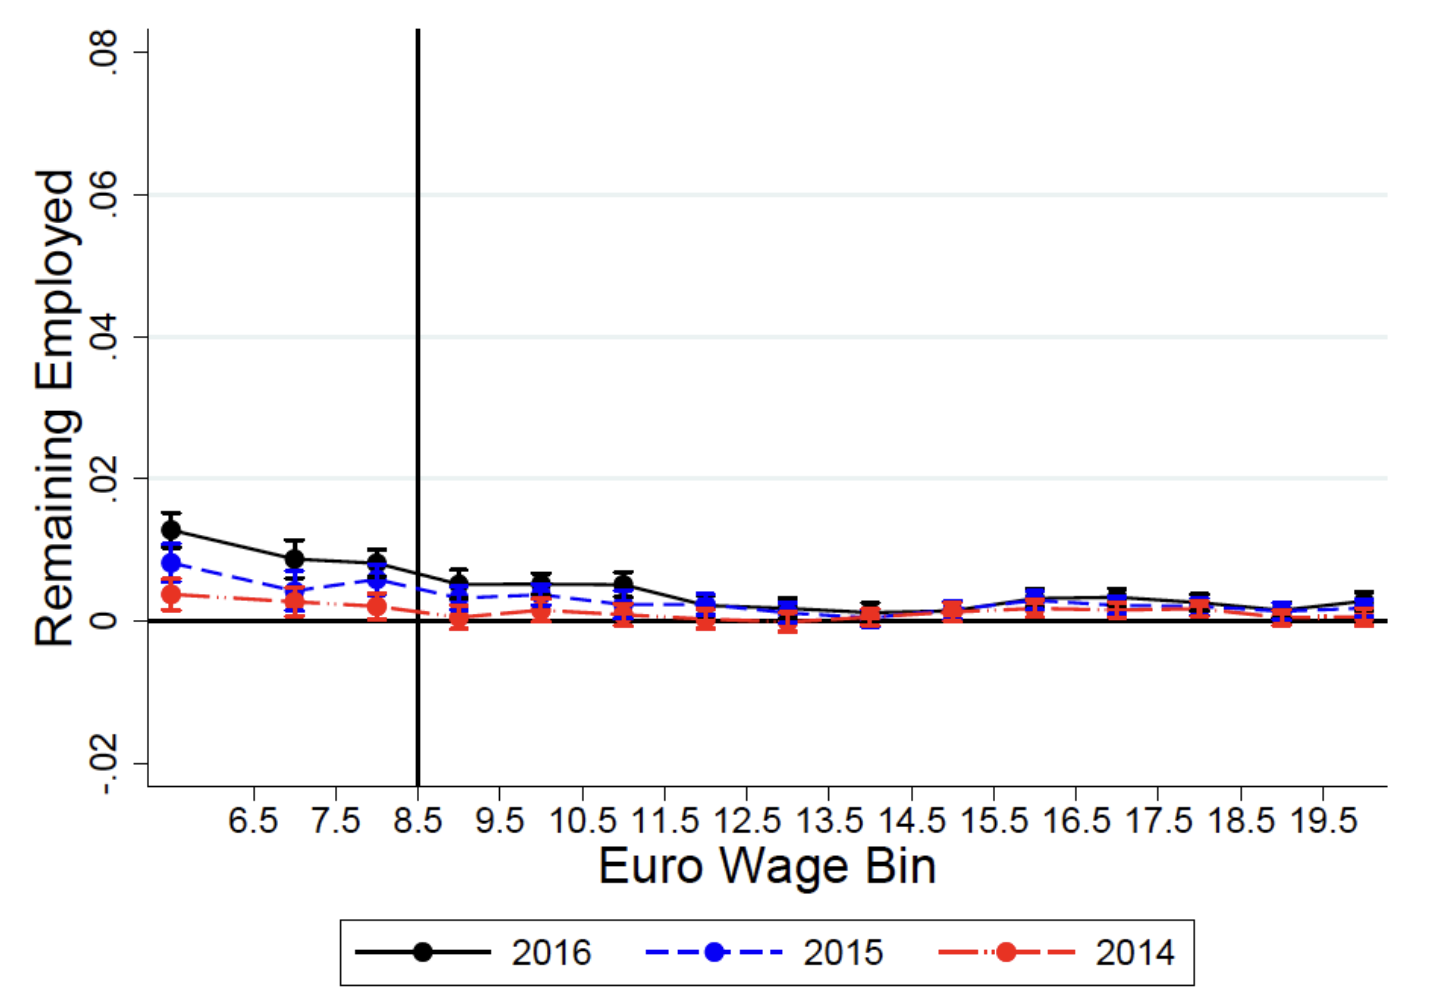
\includegraphics[width=4in]{images/ch2/reallocation_2.png}
                \caption{Employment Growth as a Function of Employment 2 Years Before}
            \end{figure}
            Higher wage premium:
            \begin{figure}[H]
                \centering
                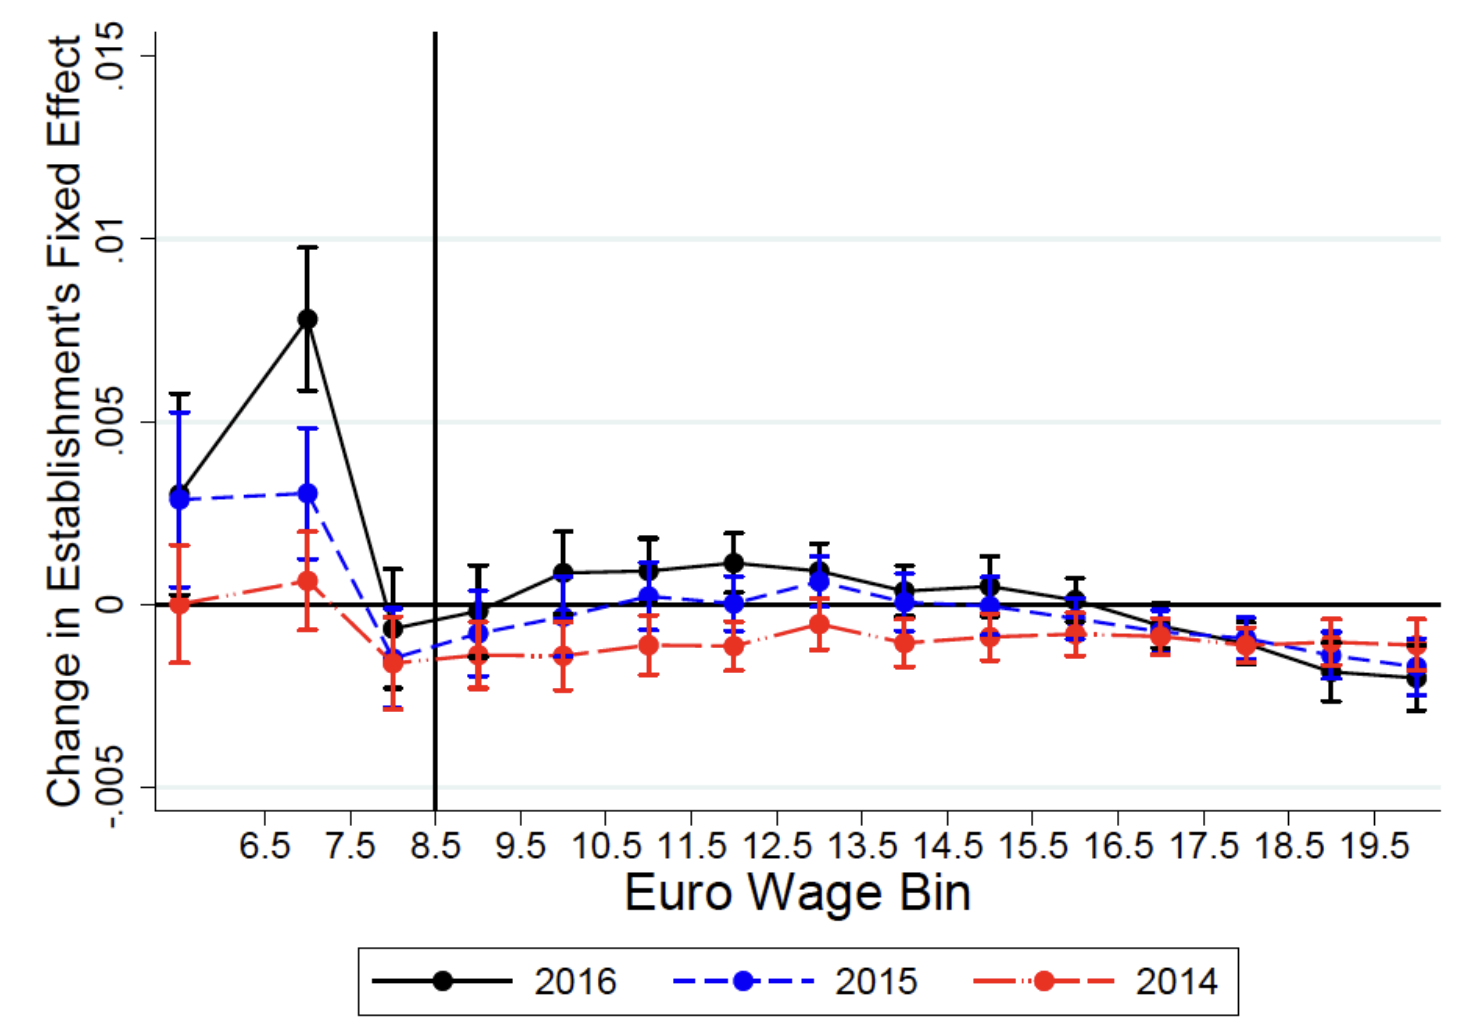
\includegraphics[width=4in]{images/ch2/reallocation_3.png}
                \caption{Firm Wage Premium as a Function of Wages 2 Years Before}
            \end{figure}
            Higher productivity:
            \begin{figure}[H]
                \centering
                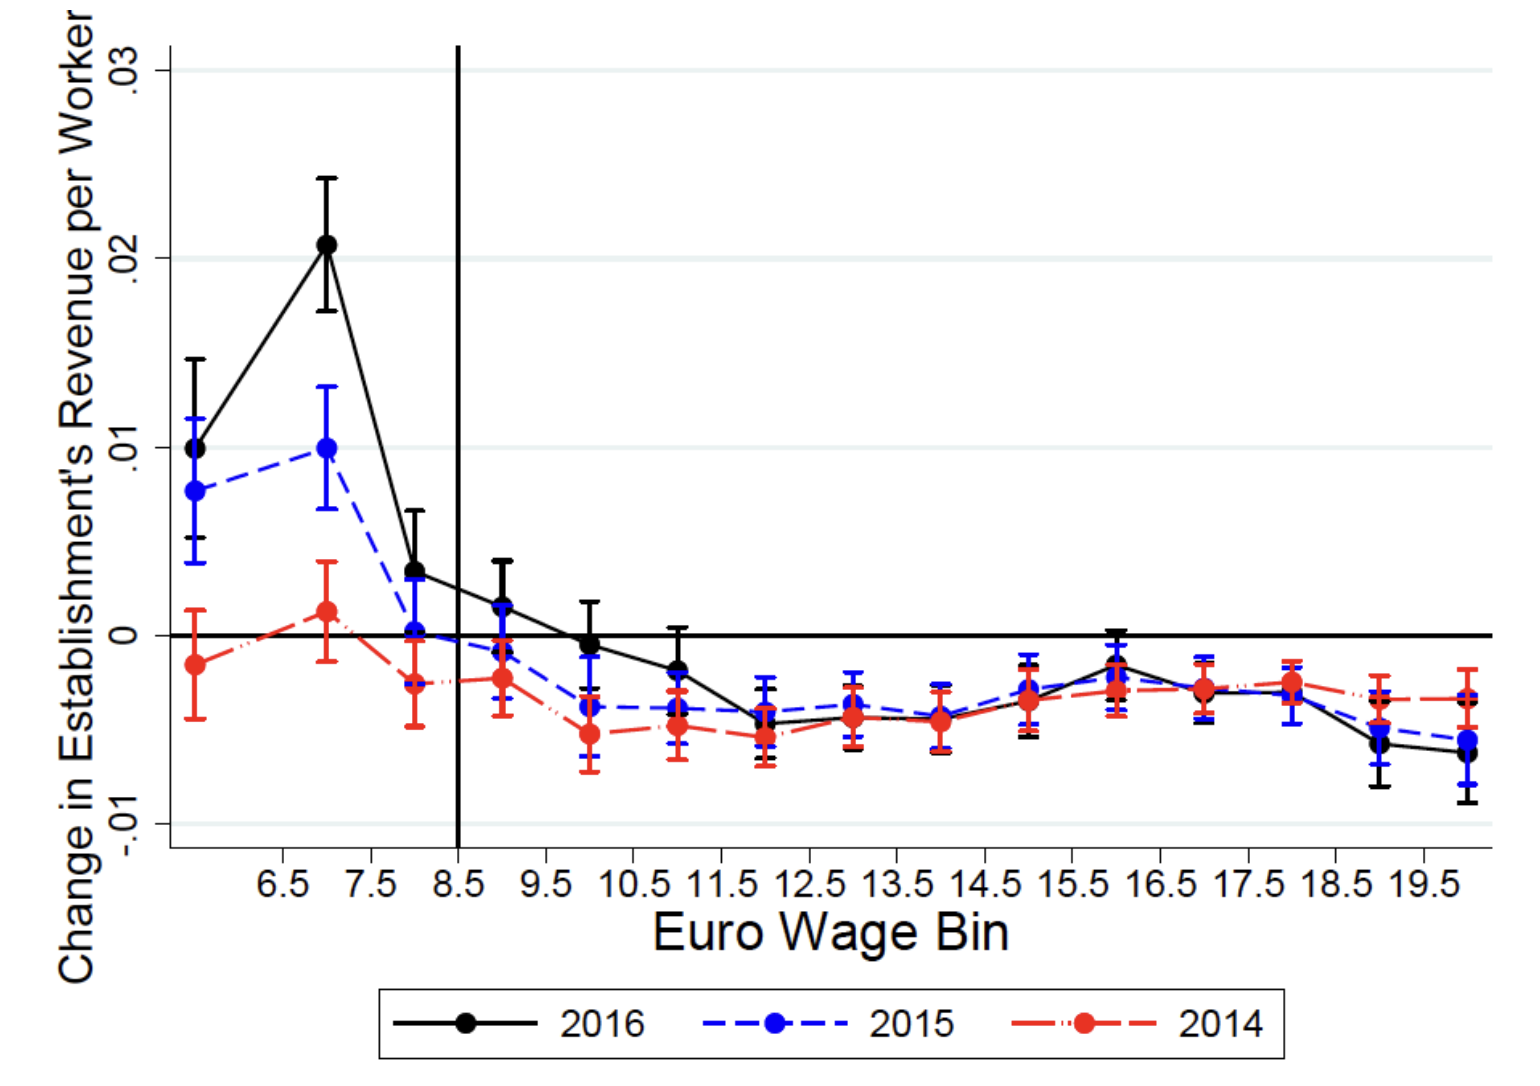
\includegraphics[width=4in]{images/ch2/reallocation_4.png}
                \caption{Firm’s Productivity Growth as a Function of Wages 2 Years Before}
            \end{figure}
            Reallocation from small firms to larger firms:
            \begin{figure}[H]
                \centering
                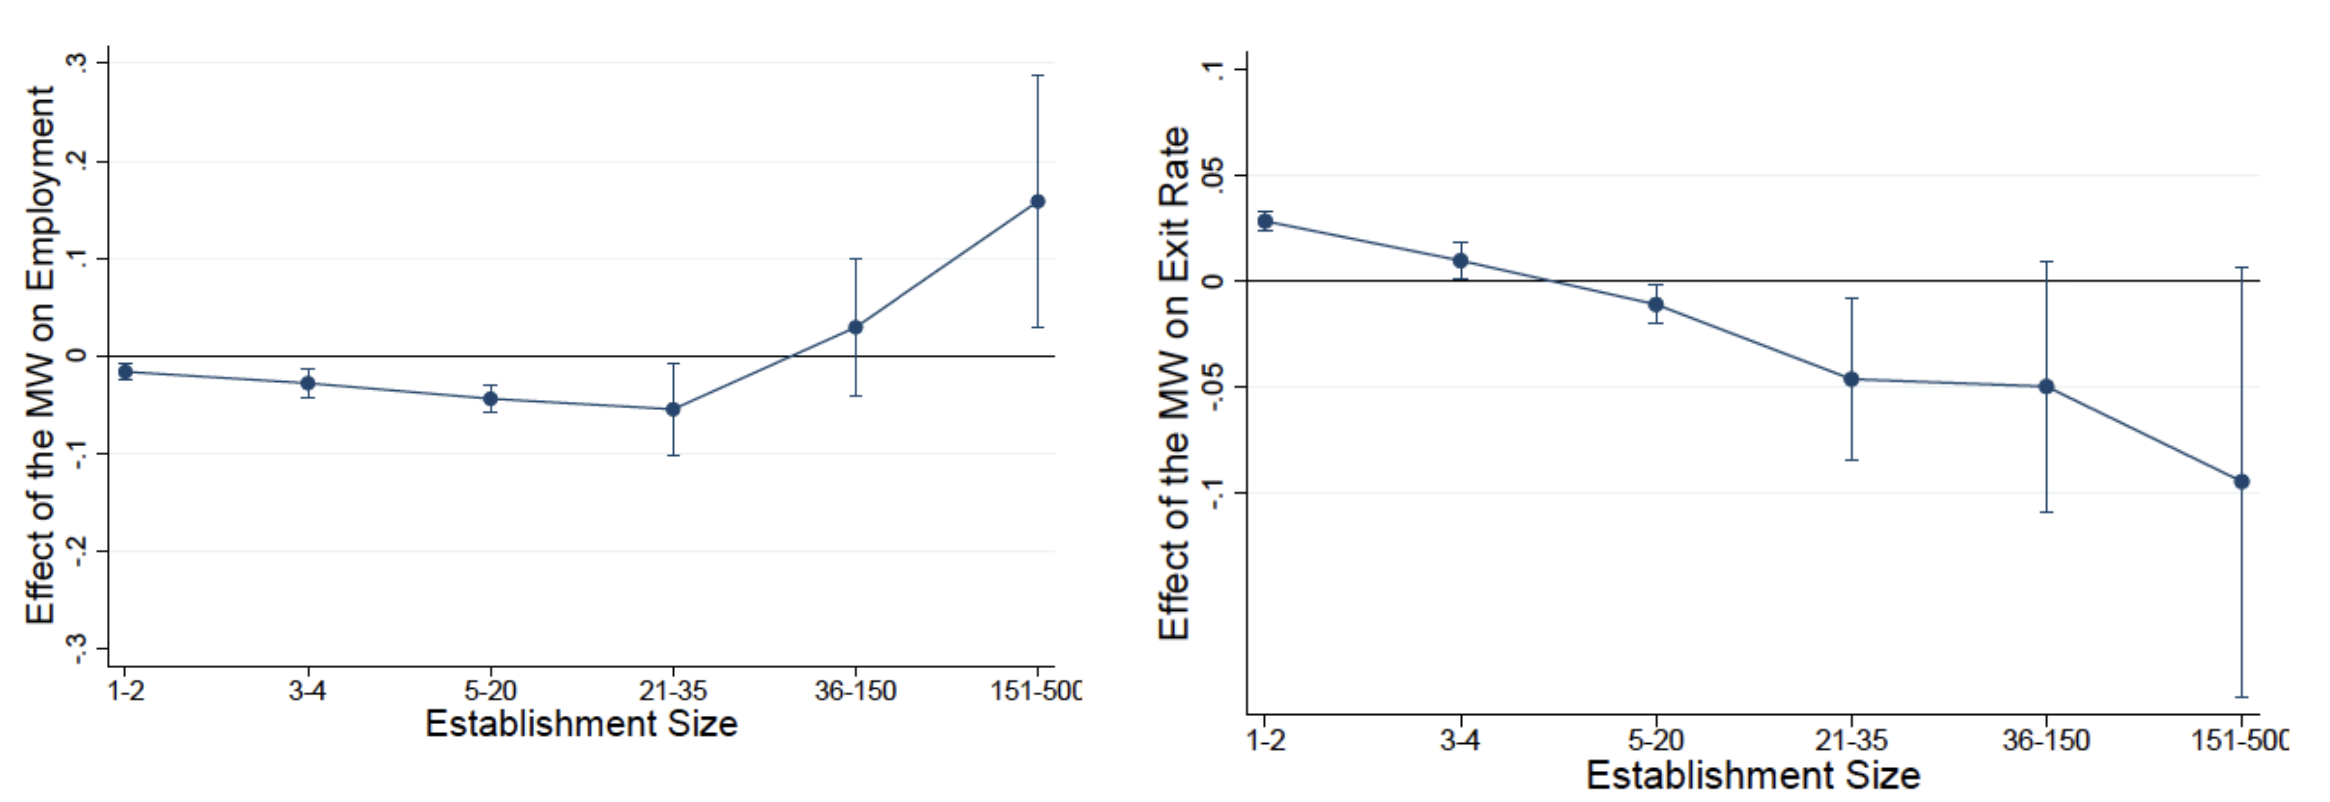
\includegraphics[width=5.5in]{images/ch2/reallocation_5.png}
                \caption{The Effect of the Minimum Wage by Firm Size}
            \end{figure}
            Key findings:
            \begin{itemize}
                \item Positive and significant effect on wages
                \item No dis-employment effect
                \item \emph{Reallocation} of workers to:
                \begin{itemize}
                    \item Firms paying higher wage premium
                    \item Firms with lower turnover
                    \item Firms with larger sizes higher productivity
                \end{itemize}
            \end{itemize}
            This indicates that minimum wages reallocate workers to more productive firms, contributing productivity improvement. The welfare implication is more ambiguous since there's evidence that workers' commuting distance increased.